\section{Modular categories}
\label{modular-categories}

\subsection{Overview}

\subsubsection{Introduction}

In this chapter we will be giving a detailed analysis of modular categories, the abstract algebraic structures used to describe anyons in topological order. We recall below how this fits into the general framework of this book:

\begin{equation*}
\tikzfig{mathematical-outline-MTC}
\end{equation*}

Describing exactly what an anyon is and how it can transform in terms of states and unitary operators on a Hilbert space can be difficult. However, describing abstractly how these transformations compose with one another can be done realtively simply. Hence we take a composition-first category-theoretic approach to anyons. We will make heavy use of the diagramatic language of braided monoidal categories established in chapter \ref{category-theory}. Roughly, we can think of a modular category as being the category with the following data:

\begin{equation*}
\left(\substack{
\mathbf{objects:}\text{ finite collections of anyons}\\
\mathbf{morphisms:}\text{ motions/behaviors of anyons}
}\right)
\end{equation*}

We have the following general pictuture for our algebraic theory:

\begin{dict}\label{topo-phase-dictionary} Topological phases of matter are algebraically described by unitary modular categories $\cC$ called the {\em anyon theory} of the phase, and a choice of integer $c_-\in \bZ$ called the {\em chiral central charge} of the phase. \cite{kitaev2006anyons}
\end{dict}

\begin{rem}\label{chiral-central-charge-remark} Throughout these notes, there are some aspects of the general dictionary \ref{topo-phase-dictionary} that we have not emphasized. For instance, we have not emphasized that the modular categories describing topological phases are supposed to be {\em unitary} modular categories - we will discuss this later, but by analagy we can say that a unitary modular category is related to a modular category just like a Hilbert space is related to a vector space.

Another aspect we have not emphasized is the {\em chiral central charge}. This is a real invariant of topological phases which is beyond the description of modular categories. In particular, there are topological phases with no non-trivial anyons (and hence correspond to the trivial modular category) yet are non-trivial as topological phases. These are called {\em invertible} topological phases. Invertible topological phases are paramaterized by an integer invariant, their chiral central charge. Not every pair $(\cC,c_-)$ describes a valid topological phase. In particular, $\cC$ determines $c_-$ modulo $8$ but there is no other condition. The way that $\cC$ determins $c_-$ modulo $8$ is known as the Gauss-Milgram formula and is discussed in subsection \ref{vafa-theorem-unitarity-chiral-central-charge}. 
\end{rem}

\begin{rem}
The major structures of a modular tensor category can be motivated by considering abstractly the possible motions and behaviors of anyons. The most basic thing anyons can do is move anyons around each other - this is known as {\em braiding}. If the anyons touch each other then they can congeal into a single  anyon - this is known as {\em fusion}. Even if there are no anyons in a system, however, there is always something possible. Anyons can be spontaneously created, so long as every anyon which is created comes along with its corresponding antiparticle. This is known as {\em pair-creation}. These three operations are the fundamental structures which we will building into modular categories:

\begin{enumerate}
\item braiding;
\item fusion;
\item pair-creation.
\end{enumerate}
\end{rem}

\begin{rem}
Another potentially useful way of thinking about modular categories comes from analogy with classical physics. We saw in chapter \ref{overview} that topological classical systems have an algebraic description in terms of finite groups. Namely, quasiparticles in the system of ordered media with order space $M$ is algebraically characterized by the fundamental group $\pi_1(M,m)$ of $M$ relative to some basepoint $m\in M$. Seeing as topological order is a vast quantum generalization of classical ordered media, we can think of modular categories as being a vast quantum generalization of finite groups. Every finite group $G$ induces a modular category $\fD(G)$, by first constructing the Kitaev quantum double model based on that finite group and then describing its anyons. Many modular categories do not come from the group-theoretical construction.
\end{rem}

\subsubsection{Using the final product}

Before developping the theory of modular categories, it is good to get a feel for what using the final product is like. A modular category itself will be a big infinite structure, with infinitely many objects and infinitely many morphisms between those objects. However, all modular categories are in a real sense {\em finitely generated}. What we mean by this is that plugging in a finite number of objects and morphisms, the rest of the obejcts and morphisms can be recovered by the abstract rules encoded in the formalism. In this way, the axioms of modular categories are not only neccecary by the fact that they restrict which categories can be modular categories, but they are also vital in the fact that they allow us to generate a full description of anyons from a minimal collection of data. For practically-minded readers, this can be viewed as the main motivation for putting so much work into defining modular categories..

\begin{ex}
To highlight how the formalism used to define an object impacts its finitely-generated description, we take an example from group theory. Consider the 3-strand braid group $B_3$. This group has ininitely many elements and the group operation $B_3\times B_3\to B_3$ naively takes an infinite amount of data to describe. However, the presentation

$$B_3=\Braket{\sigma_1, \sigma_2 | \sigma_1 \sigma_2 \sigma_1 = \sigma_2 \sigma_1 \sigma_2}$$

gives  completely finite description of $B_3$. It is important to note, however, that this presentation would {\em not} have been enough to recover $B_3$ if we had just been told that $B_3$ is a monoid. The fact that $B_3$ is a group implied the existence of elements $\sigma_1^{-1}$, $\sigma_{2}^{-1}$, and defined how they interacted with $\sigma_1,\sigma_2$. We see in this way that the axioms of a group not only serve as a restriction on what mathematical objects are allowed to be groups, but they also serve as a compression technique. They give the rules by which a minimal collection of data can be used to generate the rest.
\end{ex}


An important step in going from modular categories to their description in terms of a finite set of data is in comming up with an efficient standard way of descrbing morphisms in a modular category. This is done using skeletonization, as discussed in section \ref{skeletonization}. A large table of these descriptions are found in appendix \ref{anyon-data}. We now give a worked example of how this data is used to compute observable quantities.

\begin{ex}
\Note{add toric code modular category data}
\end{ex}

\begin{ex}
Or, for a more complicated example, we can consider the data for $G=S_3$:
\Note{add $G=S_3$ modular category data}
\end{ex}

\subsection{First properties}

\subsubsection{Definition}

In this section we define modular categories, which are the main mathematical subject of this book. Seeing as lots of data is involved, we spread out the definition over a series of steps as to not overload the senses. These intermediate definitions are also important in their own right, because they will be used in other places in the algebraic theory of topological phases.


\begin{defn}[Fusion category] A fusion category is the following data:

\begin{enumerate}
\item A category $\cC$;
\item The structure of a right-rigid monoidal category on $\cC$;
\item The structure of a $\bC$-linear category on $\cC$.
\end{enumerate}

Such that:

\begin{enumerate}
\item The tensor product functor $\otimes: \cC\times \cC\to \cC$ induces bilinear maps hom-spaces;
\item There is an equivalence $\cC \simeq \Vec_\bC^n$ as $\bC$-linear categories;
\item $\End_\cC(\bone)\cong \bC$ as $\bC$-vector spaces
\end{enumerate}


\end{defn}

\begin{rem}
A fusion category is part of the way towards having all of the requisite structures of a modular category: it has a method for fusion inherited from the tensor product, and it has half of a method for pair-creation coming from right-rigidity. The $\bC$-linearity allows us to think of hom-spaces as vector spaces, which allows us to treat hom-spaces as quantum systems. The condition (1) is a comptability between the $\bC$-linear structure and the monoidal structure. The conditions (2)-(3) are strong niceness and finiteness conditions - we will explain them in detail later.
\end{rem}

\begin{defn}[Spherical fusion category]\label{spherical-cat-definition} A spherical fusion category is the following data:

\begin{enumerate}
\item A fusion category $\cC$;
\item A left-rigid structure on $\cC$.
\end{enumerate}

Such that:

\begin{enumerate}
\item The left-rigid and right-rigid structures on $\cC$ satisfy the axioms of a pivotal structure on $\cC$;
\item For every object $A\in \cC$ and for every morphism $f: A \to A$, we have

\begin{equation*}
\tikzfig{spherical-category}
\end{equation*}
\end{enumerate}
\end{defn}

\begin{rem}
A spherical fusion category now has a structure for fusion, and a full structure for pair-creation. The 2nd axiom in definition \ref{spherical-cat-definition} is known as the {\em spherical axiom}. We will explain this axiom in more detail later.
\end{rem}

\begin{defn}[Pre-modular category] A pre-modular category is the following data:

\begin{enumerate}
\item A spherical fusion category $\cC$;
\item A braided structure on $\cC$.
\end{enumerate}

No extra compatibility conditions are required.
\end{defn}

\begin{rem}
A pre-modular category has all of the structure we require of a modular category: fusion, pair-creation, and braiding. The final axiom it is missing is a non-degeneracy condition. The non-degeneracy condition is subtle in its interpretation, and we will explain it several different ways throughout this chapter.
\end{rem}

\begin{defn}[Modular category] A modular category is a pre-modular category satisfying the following condition. Let $A\in \cC$ be an object. If

\begin{equation*}
\tikzfig{non-degeneracy}
\end{equation*}

for all $B\in \cC$, then $A\cong n\cdot \bone$ for some $n\geq 1$.
\end{defn}

\begin{rem} Our usage of the term ``modular category" is a bit nonstandard. Where we call ``modular categories" most authors would call ``modular {\em tensor} categories". I find ``modular category" more convient here because it is shorter than ``modular tensor category" and I want to be succinct. For many authors, the term ``modular category" refers to a potentially non-semsimple modular category, such as in Turaev's original work on modular categories \cite{turaev1992modular}.
\end{rem}

\begin{ex}\label{modular-category-examples} The category $\Vec_{\bC}$ is naturally a modular category. We discusses its $\bC$-linear structure in example \ref{linear-category-examples}, we discussed its pivotal structure in subsection \ref{pivotal-category-examples}, and we discussed its braided monoidal structure in examples \ref{monoidal-category-examples}, \ref{braided-monoidal-examples}. It satisfies $\Hom_{\Vec_{\bC}}(\bC,\bC)\cong \bC$, the right-rigid structure and the $\bC$-linear structure turn $\Vec_{\bC}$ into a fusion category. As we saw in example \ref{pivotal-category-examples}, the fusion category structure and the left-rigid structure turn $\Vec_{\bC}$ into a spherical fusion category.  Clearly $\Vec_{\bC}$ satisfies the non-degeneracy axiom, because every object is isomorphic to $n\cdot \bone$ for some $n\geq 1$! Thus, $\Vec_{\bC}$ is indeed a modular category.
\end{ex}

\begin{dict} The category $\Vec_{\bC}$ equipped with chiral central charge $c_-=0$ corresponds physically to the {\em trivial phase}. That is, the phase of matter describing empty space.
\end{dict}

\subsubsection{Anyons in modular categories}

Modular categories are supposed to be theories of anyons in topological order. So, now that we have the definition of modular category, it is natural to ask: what do anyons mathematically correspond to, in modular categories? The answer lies within the condition in a fusion category $\cC$ that there is an equivalence $\cC\cong \Vec_\bC^n$ as $\bC$-linear categories. We saw in proposition [ref] that every object $A\in \cC$ is isomorphic to a direct sum of {\em simple objects}, objects which cannot be written as the direct sum of two nonzero objects. Alternatively, $A\in \cC$ is simple if and only if $\End(A)\cong \bC$.

\begin{dict}\label{anyon-types-definition}
Isomorphism classes of simple objects in $\cC$ correspond to anyon types in a topological phase described by the MTC $\cC$.
\end{dict}

\begin{defn} For all fusion categories $\cC$, we define $\cL(\cC)$ (or simple $\cL$ when $\cC$ is clear from context) to the the set of isomorphism classes of simple objects. By entry \ref{anyon-types-definition} of the physics-math direction, elements of $\cL(\cC)$ correspond bijectively to anyon types in any topological phase described by $\cC$.
\end{defn}

We now restate the results of proposition \ref{higher-linear-algebra} in our current setting for a fusion category $\cC$.  For every object $X\in \cC$, there exists unique nonnegative integers $c_{[A]}$, $[A]\in \cL$, such that

$$X\cong \bigoplus_{[A]\in \cL}c_{[A]}\cdot A.$$

We assumed in the definition of a fusion category that $\End_\cC(\bone)\cong \cC$. Thus, the monoidal unit is a simple object in every fusion category. By our physics-math dictionary, this means that $\bone$ corresponds to an anyon type. This anyon $\bone$ is the trivial ``no-anyon" type, corresponding to a quasiparticle which happens to be the same as the homogenous bulk.

\begin{dict}\label{vacuum-anyon-definition} The monodial unit $\bone $ corresponds to the trivial anyon type, which is the same as the homogenous bulk (sometimes called the  {\em vaccuum} anyon type).
\end{dict}

\begin{rem} Continuing in our expansion of the physics-math dictionary, we can assert that dual objects (defined using the right-rigid structure on a fusion category) correspond to antiparticles (entry \ref{antiparticle-definition}). This is consistent with the fact that anyon types correspond to simple objects, by proposition \ref{simple-dual-simple}.
\end{rem}

\begin{dict}\label{antiparticle-definition}
For every simple object $A$ in a modular category $\cC$, the dual object $A^*$ corresponds to the {\em antiparticle} of $A$.
Expanding our physics-math dictionary, we say that for every anyon $A$ its {\em antiparticle} is the dual $A^*$ which comes from right-rigidity. This gives a valid anyon type by proposition \ref{simple-dual-simple}.
\end{dict}

\begin{prop}\label{simple-dual-simple} Let $\cC$ be a fusion category. If $A\in \cC$ is a simple object, then so is $A^*$.
\end{prop}
\begin{proof} By proposition \ref{rigidity-functorial} duality induces a bijection on hom-spaces. Since composition is bilinear, duality is thus an isomorphism of vector spaces on all hom-spaces. Hence, for all $A\in \cC$ there is an isomorphism $\Hom(A,A)\cong \Hom(A^*,A^*)$.  So, $\dim \Hom(A,A)= 1$ if and only if $\dim \Hom(A^*,A^*)=1$, and thus the result follows from Schur's lemma.
\end{proof}

\begin{dict}\label{composite-system-def}
The tensor product $\otimes$ physically corresponds to joining anyons, forming a composite anyon configuration. That is, the object $A\otimes B$ corresponds to the configuration with one $A$-type anyon and one $B$-type anyon.
\end{dict}

\begin{rem} By entry \ref{composite-system-def} of the physics-math dictionary and proposition \ref{fusion-category-simples}, it behooves us to take a moment to interpret the direct sum decomposition

\begin{equation}
A\otimes B \cong \bigoplus_{[C]\in \cL}N^{A,B}_{C}\cdot C,
\end{equation}

where $A,B\in \cC$ are objects in a fusion category. We call the non-negative integers $N^{A,B}_C$ the {\em fusion coefficients} of $\cC$. We observe that

\begin{equation}\label{fusion-rule-dimensions}
\dim \Hom(A\otimes B, C)=N^{A,B}_C.
\end{equation}

Morphisms in $\cC$ correspond to physical processes. So, equation \ref{fusion-rule-dimensions} can be interpreted as saying that whenever $N^{A,B}_{C}>0$, there is a physical process $A\otimes B\to C$. That is, there is a physical process which goes from the composite system of one $A$-type anyon and one $B$-type anyon and ouputs one $C$-type anyon. Neccecarily, such a process can be interpreted as {\em fusion} of $A$ and $B$ to $C$. Moreover, equation \ref{fusion-rule-dimensions} tells us that the space of possible physical processes which fuse $A$ and $B$ to $C$ (known as {\em fusion channels} $A\otimes B\to C$) is $N^{A,B}_C$-dimensional.
\end{rem}

\begin{rem}\label{no-transparent-anyons}
We can interpret the modularity axiom in terms of anyons. To begin, we observe the algebraic fact that a pre-modular category is modular if and only if for all {\em simple} objects $A\in \cC$,

\begin{equation*}
\tikzfig{non-degeneracy}
\end{equation*}

for all {\em simple} objects $B\in \cC$ implies $A\cong \bone$. This is physically interpreted as saying that if an anyon braids trivially with all other anyons, then it must be the trivial anyon type $\bone$. In otherwords, there are no {\em transparent} anyons. This fact is physically motivated in subsection [ref].
\end{rem}

\begin{prop} Let $\cC$ be a fusion category. For all simple objects $A,B,C,E\in \cC$,

\begin{equation}
\sum_{E}N^{A,B}_{E}N^{E,C}_{D}=\sum_{G}N^{B,C}_{G}N^{A,G}_{D}.
\end{equation}
\end{prop}
\begin{proof} We observe on one hand that

\begin{align*}
(A\otimes B)\otimes C& \cong \bigoplus_{E}N^{A,B}_{E}\cdot E\otimes C\\
&\cong \bigoplus_{E,D}N^{A,B}_{E}N^{E,C}_{D}\cdot D
\end{align*}

and on the other hand

\begin{align*}
A\otimes (B\otimes C)& \cong \bigoplus_{G}N^{B,C}_{G}\cdot A\otimes G\\
&\cong \bigoplus_{G,D}N^{B,C}_{G}N^{A,G}_{D}\cdot D.
\end{align*}

Since $(A\otimes B)\otimes C\cong A\otimes (B\otimes C)$, we can compare coefficients to get the result.
\end{proof}

\begin{prop} Let $\cC$ be a braided fusion category. For all simple objects $A,B,C$,

\begin{equation}
N^{A,B}_{C}=N^{B,A}_{C}.
\end{equation}
\end{prop}
\begin{proof} This follows immediately from the fact that $A\otimes B\cong B\otimes A$ in a braided fusion category.
\end{proof}


\subsubsection{States in modular categories and unitarity}

It is now worth reflecting on how to interpret states in a topologically ordered system in terms modular categories. Certainly, objects in modular categories do {\em not} correspod quantum systems. They don't have vector space structure. Objects correspond roughly to anyon configurations, which are classical observables. The hom-spaces are what have vector space structure, by $\bC$-linearity. However, they are not yet Hilbert spaces. It is exactly for this reason we need to define {\em unitary modular categories}. These are modular categories in which hom-spaces have Hilbert space structure.

\begin{defn}[Unitary fusion category] A unitary fusion category is the following data:

\begin{enumerate}
\item An fusion category $\cC$.
\item (Conjugation) A linear map $\dagger: \Hom(A,B)\to \Hom(B,A)$ for all $A,B\in \cC$.
\end{enumerate}

Such that:

\begin{enumerate}
\item (Unitarity) Given $f:A\to A$ an endomorphism of $A\in \cC$, define


$$\tr(f)=\ev_A \circ (\id_{A^*}\otimes f)\circ \left(\ev_A\right)^{\dagger}.$$

The map $\left<\cdot|\cdot\right>:\Hom(A,B)\times \Hom(A,B)\to \bC$ defined by $\left<f|g\right>=\tr(f^{\dagger}\circ g)$ is an inner product, endowing $\Hom(A,B)$ with the structure of a Hilbert space.
\item $\left(f^{\dagger}\right)^{\dagger}=f$ for all $f\in \Hom(A,B)$, $A,B\in \cC$.

\item $(f\circ g)^{\dagger}=g^{\dagger}\circ f^{\dagger}$ for all $f\in \Hom(B,C)$,$g\in \Hom(A,B)$, $A,B,C\in \cC$.

\item $(f\otimes g)^{\dagger}=f^{\dagger}\otimes g^{\dagger}$ for all $f\in \Hom(A,B)$,$g\in \Hom(C,D)$, $A,B,C,D\in \cC$.
\item $\left(\coev_A\right)^{\dagger}\circ (f \otimes \id_{A^*})\circ \coev_A=\tr(f)$ for all $A\in \cC$
\end{enumerate}
\end{defn}

\begin{rem}
Unitary fusion categories make for a pleasant object of study because by proposition \ref{UFC-pivotal} the distinguished maps $(\ev_A)^{\dagger}:1\to A^{*}\otimes A$ and $(\coev_A)^{\dagger}:A\otimes A^{*}\to 1$ induce a pivotal structure.
\end{rem}

\begin{rem} In subsection [ref] proposition \ref{UFC-pivotal}, we will show that in every unitary fusion category the maps $\ev_{A}^L = (\coev_{A})^{\dagger}$ and $\coev^L_{A}=(\ev_A)^{\dagger}$ give a left-rigid structure on $\cC$. This left-rigidity endows $\cC$ with the structure of a spherical fusion category. Thus, every unitary fusion category is automatically a spherical fusion category.
\end{rem}

\begin{defn}[Unitary pre-modular category] A unitary modular category is the following data:

\begin{enumerate}
\item A modular category $\cC$;
\item (Conjugation) A linear map $\dagger: \Hom(A,B)\to \Hom(B,A)$ for all $A,B\in \cC$.
\end{enumerate}

Such that:

\begin{enumerate}
\item Forgetting the left-rigid structure and braiding, $\left(\cC,\dagger\right)$ forms a unitary fusion category.
\item $\left(\ev_{A}^R\right)^{\dagger}=\coev_{A}^L$;
\item $\left(\coev_{A}^R\right)^{\dagger}=\ev_{A}^L$;
\item $\left(\beta_{A,B}\right)^{\dagger}=\beta_{B,A}^{-1}$.
\end{enumerate}
\end{defn}

\begin{defn}[Unitary modular category] A unitary modular category is a unitary pre-modular category which satisfies the non-degeneracy axiom of a modular category.
\end{defn}

\begin{rem} The compatibility conditions for the twist are chosen so that the definition of trace as a modular category and the definition of trace as a unitary fusion category coincide.
\end{rem}

\begin{dict} For any phase whose anyons as described by a unitary modular category $\cC$.

\begin{equation}\label{dict-state-formula}
\left(\substack{\text{states of topological order $\cC$} \\ \text{on the sphere $S^2$} \\ \text{with anyon configuraiton $A_1,A_2...A _n$}}\right)
=
\left(
\substack{
\text{normalized vectors in the Hilbert space}\\
\Hom_\cC(\bone, A_1\otimes A_2... \otimes A_n)
}
\right)
\end{equation}

where by ``anyon configuration $A_1,A_2...A_n$" we mean that the state has anyons present in $n$ sites, arranged left to right on a line segment in the sphere, with corresponding anyon type $A_1,A_2...A_n$.
\end{dict}

\begin{rem} It is not immediately clear why the physical space in equation \ref{dict-state-formula} should be there sphere. As one source of motivation, we can observe the following corollary of equation \ref{dict-state-formula}:

\begin{equation*}
\dim\left(\substack{\text{Hilbert space of topological order $\cC$} \\ \text{on the sphere $S^2$} \\ \text{with exactly one anyon of type $A$}}\right)
=
\dim \Hom(\bone, A)
=
\begin{cases}
1 & A=\bone \\ 
0 & \text{otherwise}.
\end{cases}
\end{equation*}

Hence, we conclude that if the sphere has exactly one anyon on it then that anyon type must be trivial. Moreover, there is unique state on the sphere with no anyons. This is true on physical grounds. Suppose there was a state on the sphere with a single anyon of type $A$. Now choose any other anyon $B$. We observe that braiding $B$ around $A$ acts by the phase $+1$, because the loop of $B$ can be contracted around there other side of the sphere, as illustrated in figure \ref{sphere-braiding}. Diagramatically, this means that for all simple objects $B\in \cL$

\begin{figure}[h]
\begin{center}
\includegraphics[scale=.15]{sphere-braiding}
\end{center}
\caption{Illustration of braiding around a single anyon on the sphere}
\label{sphere-braiding}
\end{figure}

\begin{equation*}
\tikzfig{non-degeneracy}
\end{equation*}

By modularity (c.f. remark \ref{no-transparent-anyons}), this implies  $A\cong \bone$. Thus, the if there is only one anyon on the sphere it must have trivial type. The fact that there is a unique state on the sphere with no anyons is also true on physical grounds, but is more subtle. It is discussed in subsection [ref].
\end{rem}

\begin{dict} For any modular category $\cC$,:

\begin{equation}\label{dict-state-formula-2}
\left(\substack{\text{states of topological order $\cC$} \\ \text{on the infinite flat plane $\bR^2$} \\ \text{with anyon configuraiton $A_1,A_2...A _n$}}\right)
=
\left(
\substack{
\text{normalized vectors in the Hilbert space}\\
\Hom_\cC\left(\bigoplus_{[B]\in \cL}B, A_1\otimes A_2... \otimes A_n\right)
}
\right)
\end{equation}
\end{dict}

\begin{rem}
Replacing $\bone$ with $\bigoplus_{[B]\in \cL} B$ reflects the differences between the sphere and the infinite flat plane. On a sphere, the only way to have a state with a single isolated anyon is for that anyon to have trivial charge. However, on the plane you can have a state with any single isolated anyon. This is done by creating a particle/antiparticle pair, and then pulling one half of that pair away to infinity, as illustrated in figure \ref{plane-state}. This is reflected by the fact that equation \ref{dict-state-formula-2} says that for all anyon types $A$,

\begin{equation}\label{dict-state-formula-2}
\dim\left(\substack{\text{Hilbert space of states of topological order $\cC$} \\ \text{on the infinite flat plane $\bR^2$} \\ \text{with a single anyon of type $A$}}\right)
=\dim\Hom\big(\bigoplus_{[B]\in \cL}B, A\big)=1.
\end{equation}

\begin{figure}[h]
\begin{center}
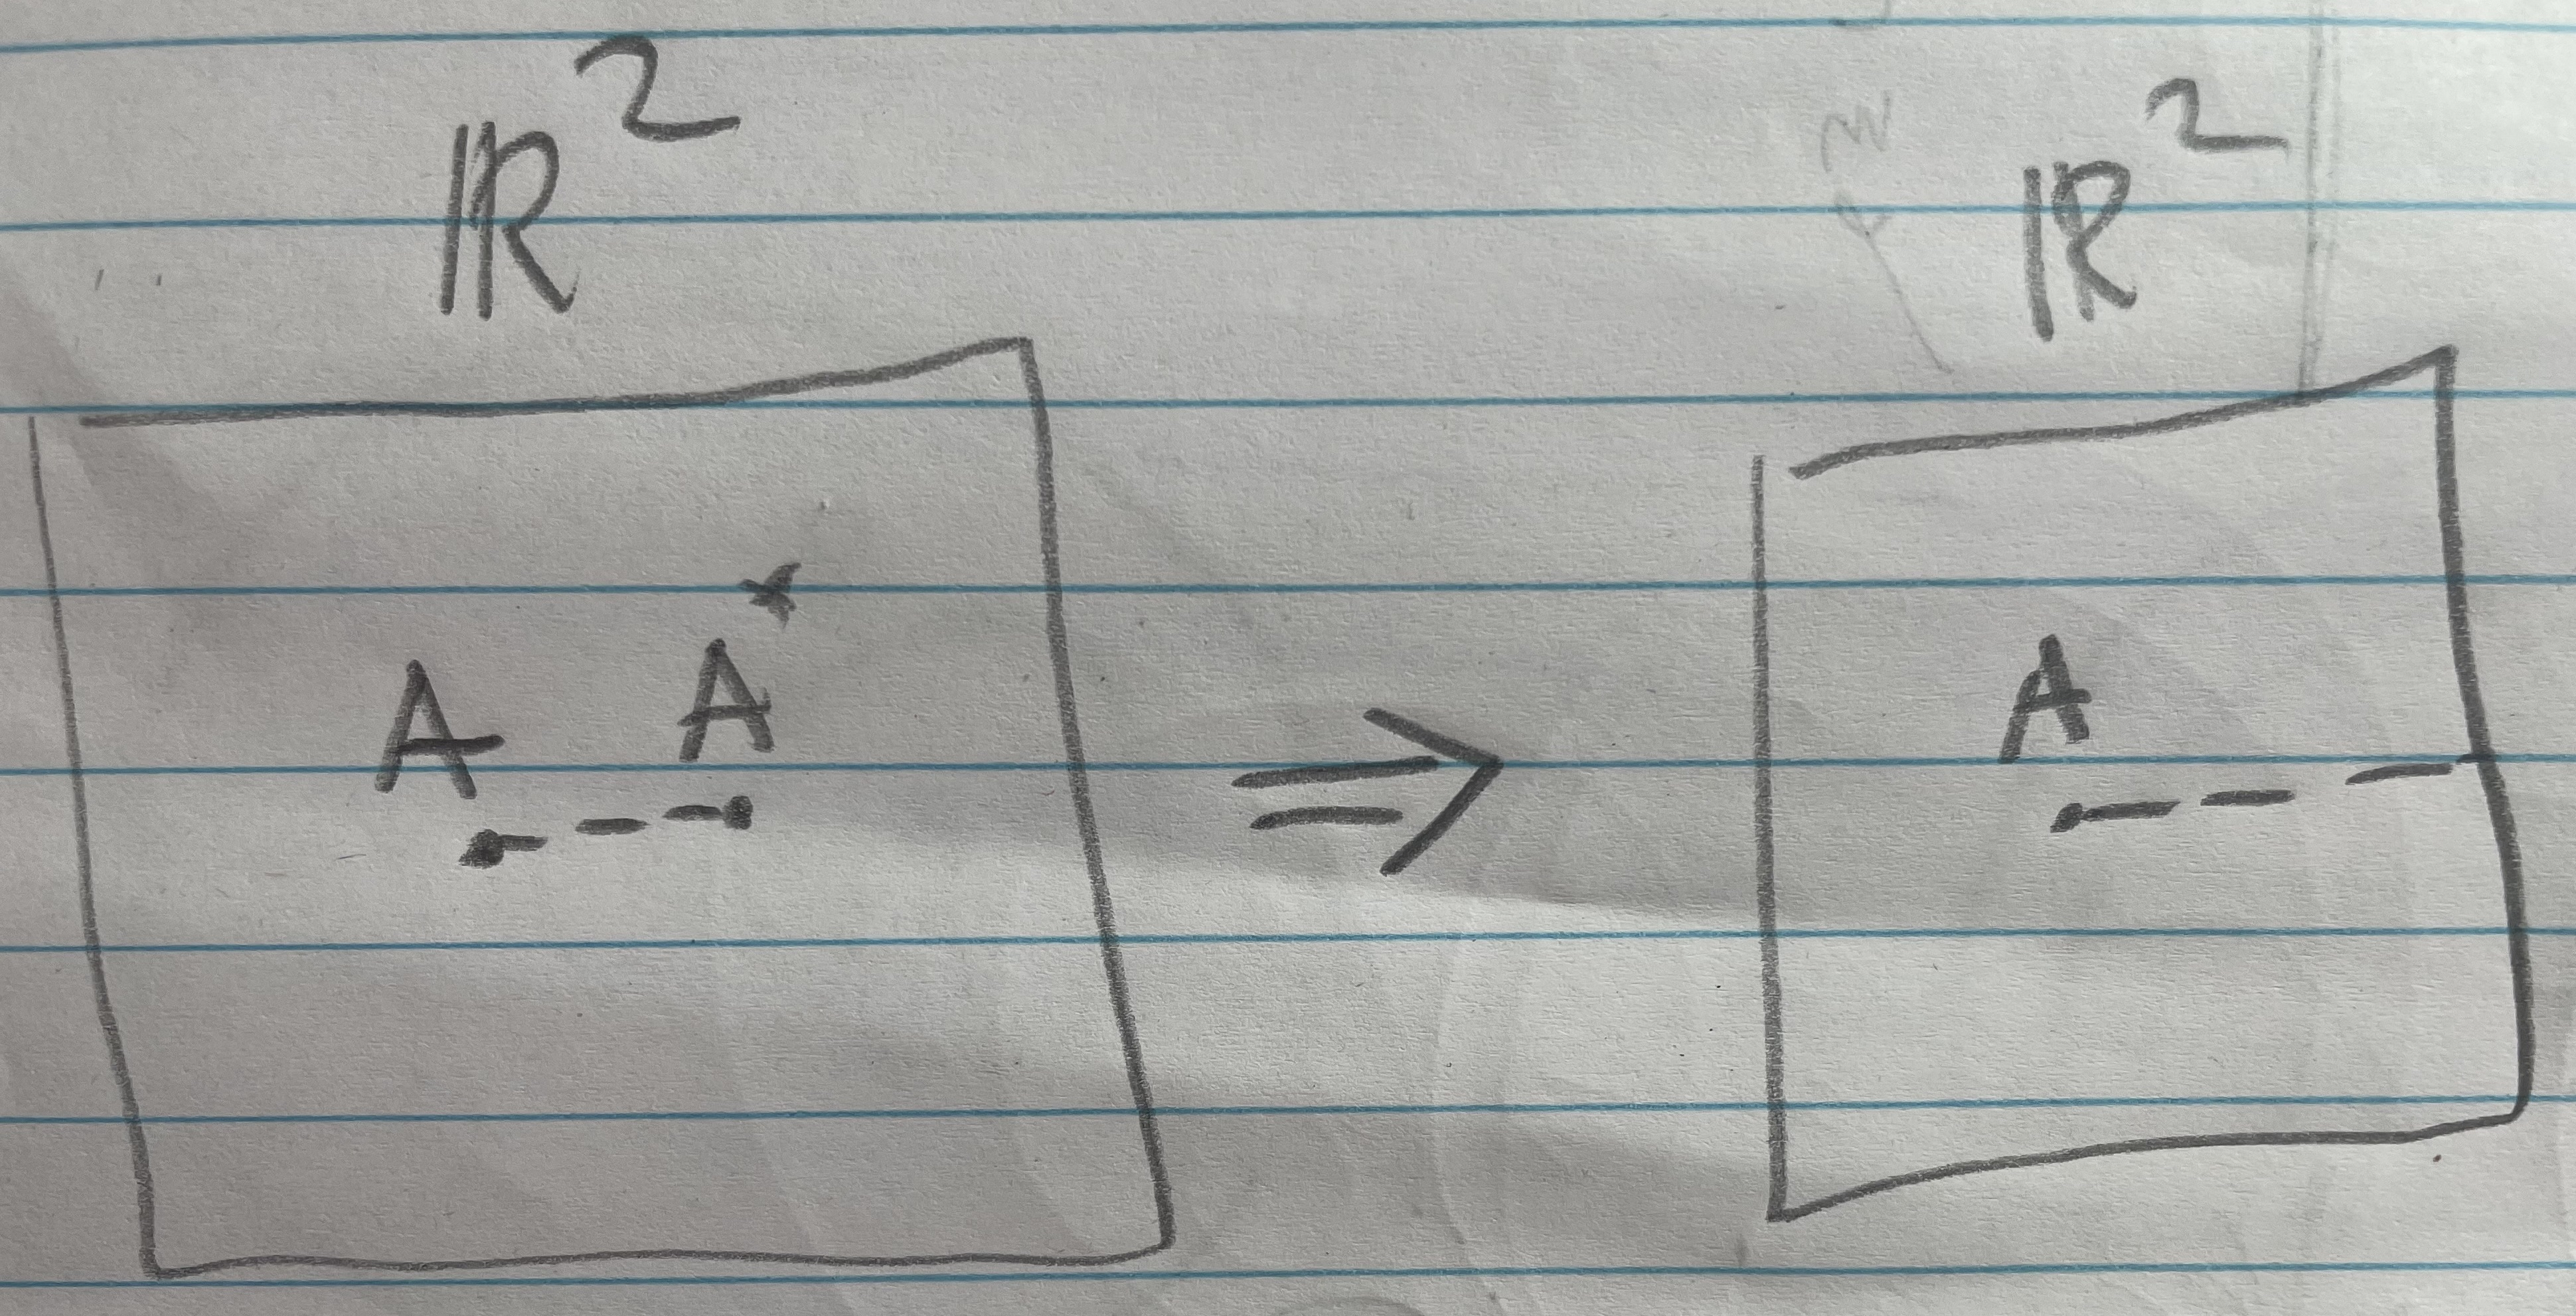
\includegraphics[scale=.035]{plane-state}
\end{center}
\caption{Creating a state on the plane with a single isolated anyon}
\label{plane-state}
\end{figure}

The fact that there is a unique state with a single anyon of type $A$ on the plane $\bR^2$ is a more subtle physical argument, discussed in subsection [ref].
\end{rem}

\begin{rem} Working on higher-genus surfaces or on surfaces with holes is possible, but it is a bit cumbersome in the approach were are taking. We refer to appendix [ref] for a discussion of the topic.
\end{rem}

\begin{rem}
The anyon configurations in equations \ref{dict-state-formula} and \ref{dict-state-formula-2} are always assumed to be linear. The main reason to do this is because it makes the mathematics much simpler. Keeping track of the positions of each of the anyons in two dimensional space adds unnececary complexity. Seeing as every anyon configuration can be pushed onto a one-dimensional space, only working with a one-dimensional configuration does not affect the generality of the answers and hence it is prefered.
\end{rem}

\begin{rem} The formula $\Hom_{\cC}(\bone, A_1\otimes A_2...\otimes A_n)$ encodes the fact that states can be specified by their history. There are multiple states with anyon configuration $A_1\otimes A_2...\otimes A_n$. One way of specifying a state $\ket{\psi}$ is to  start with the unique state on the sphere with no anyons, and then specify how $\ket{\psi}$ is constructed from the ground state via some unambigous process. This unambigous process from the state with no anyons to the state with anyons $A_1...A_n$ is a morphism in$\Hom_{\cC}(\bone, A_1\otimes A_2...\otimes A_n)$.
\end{rem}

\begin{ex} We can describe two states with four the four anyons $A,A^*,A,A^*$ as follows. The first state is obtained by starting with the unique state with no anyons, and creating two independent $(A,A^*)$ particle/antiparticle pairs adjacent to each other:

\begin{equation*}
\ket{\tikzfig{adjacent-pair}}
\end{equation*}

Another state can be constructed by creating a $(A,A^*)$ particle/antiparticle pair, then moving the halves of the pair far apart from each other, and then creating a $(A^*,A)$ particle/antiparticle pair in the space between the halves of the first pair:

\begin{equation*}
\ket{\tikzfig{nested-pair}}
\end{equation*}

These two (unnormalized) states have the same anyon configuration. However, they are distinguished by the fact that they were created by different processes. Translating pair-creation and movement into category theoretic language, we see that these two states correspond to different maps in $\Hom_{\cC}(\bone,A\otimes A^*\otimes A\otimes A^*)$.
\end{ex}

\subsubsection{Topological charge measurement}
\label{topological-charge-measurement}

In any reasonable physical theory, one needs to talk about measurements and observables. For the algebraic theory of topological quantum information, the only relevant type of measurement is a {\em topological charge measurement} \cite{bonderson2021measuring}. This is the measurement of the overall anyon type (or {\em topological charge}) of a collection of anyons. When the topological charge of a pair of anyons in a state $\ket{\psi}$ is measured, $\ket{\psi}$ will collapse onto a new state $\ket{\psi'}$ for which that pair of anyons now has a single well-defined charge as shown in equation \ref{measuring-a-pair}. That is, the two anyons will fuse together.

\begin{equation}\label{measuring-a-pair}
\tikzfig{measuring-a-pair}
\end{equation}

As a first step towards an algebraic understanding of topological charge measurement, suppose that we are presented with a normalized state on the sphere of the following form:

\begin{equation}\label{definite-charge-and-channel}
\ket{\psi}=\ket{\tikzfig{definite-charge-and-channel}}
\end{equation}

Where $A_1...A_n$, $B$ are simple objects,  and $\mu:A_1\otimes A_2\to B$ is normalized so that $\Braket{\mu | \mu}=1$. If we postcompose $\ket{\psi}$ with the map $\mu \otimes \id_{A_3\otimes...\otimes A_n}$, the result will be equal to

\begin{equation}\label{definite-charge-and-channel}
\mu^\dagger \ket{\psi}=\ket{\tikzfig{definite-charge-and-channel-2}}.
\end{equation}

This means that $\mu$ gives a physical process whereby $\ket{\psi}$ can transform to a state with an anyon of type $B$ where $A_1,A_2$ used to be. Moreover, if we postcompose $\ket{\psi}$ with $\eta\otimes \id_{A_3\otimes ... \otimes A_n}$ with any map such that $\eta\circ \mu^\dagger=0$ so $\eta \ket{\psi}$ will be zero (and thus an invalid quantum state). In particular, since there are no maps $B\to C$ for non-isomorphism simple objects $B,C$, we find that there is no physical process on the first two anyons which can be applied to $\ket{\psi}$ which results in a state with charge $C\not\cong B$ where $A_1,A_2$ used to be. This motivates the following mathematical-physical correspondance:

\begin{dict} Given a state $\ket{\psi}$ with anyon content $A_1... A_n$, $B_1... B_m$ we say that the anyons $A_1...A_n$ have overall topological charge $C$ with fusion channel $\mu:A_1\otimes A_2... \otimes A_n\to C$ if there exists $\alpha$ such that $\ket{\psi}$ can be expressed as follows:

\begin{equation}\label{definite-charge-and-channel-3}
\ket{\psi}=\ket{\tikzfig{definite-charge-and-channel-3}}
\end{equation}

If $\ket{\psi}$ is a superposition of states the form \ref{definite-charge-and-channel-3} for a fixed $C$ over different $\mu$, then we say that the anyons $A_1... A_n$ have overal topological charge $C$ but have indefinite fusion channel.
\end{dict}

\begin{prop}\label{resolution-of-id-prop} Let $A,B\in \cC$ be objects in a modular category. We have that

\begin{equation}\label{resolution-of-id}
\tikzfig{resolution-of-id}
\end{equation}

where $[C]$ runs over isomorphism classes of simple objects in $\cC$, and $\mu$ runs over any orthonomral basis of $\Hom(A\otimes B,C)$.
\end{prop}
\begin{proof} Let $f$ denote the morphism on the right hand side of equation \ref{resolution-of-id}. Choose any $[D]\in \cL$, and fusion channels $\eta,\eta':A\otimes B\to D$ in the same orthonormal basis as in equation \ref{resolution-of-id}. We have that

$$\eta'\circ f \circ \eta^\dagger=\tikzfig{resolution-of-id-proof}.$$

Seeing as there are no non-zero maps $C\to D$ for $C\not\cong D$, the only terms that survive are the ones with $C\cong D$. Moreover, since $\{\mu\}$ is chosen to be an orthonormal basis, the only term which survive are the one with $\mu=\eta=\eta'$. Thus,

$$\eta'\circ f \circ \eta^\dagger=
\begin{cases}
\id_D & \eta=\eta'\\
0 & \eta\neq \eta'.
\end{cases}$$

Similarly, the orthonormality of the basis $\{\mu\}$ gives

$$\eta' \circ \eta^\dagger=
\begin{cases}
\id_D & \eta=\eta'\\
0 & \eta\neq \eta'.
\end{cases}$$

Thus, $\eta'\circ f \circ \eta^\dagger=\eta'\circ \id_{A\otimes B} \circ \eta^\dagger$. Since $\eta$ and $\eta'$ run over bases of maps $A\otimes B\to D$,  we can take linear combinations and sums to find that $f$ and $\id_{A\otimes B}$ are equal when precomposed or postcomposed with any map. Thus, we find that $f=\id_{A\otimes B}$ as desired.
\end{proof}

\begin{cor}\label{resolution-of-id-cor} Let $\cC$ be a modular category.  For all simple objects $A_1, A_2... A_n\in \cC$, we have that 

\begin{equation}
\tikzfig{resolution-of-id-big}
\end{equation}
\end{cor}
\begin{proof} The proof follows be precomposing and postcomposing with fusion channels, completely analagously to the proof of proposition \ref{resolution-of-id-prop}.
\end{proof}

\begin{rem} Corollary \ref{resolution-of-id-cor} tells us every state $\ket{\psi}$ with anyon content $A_1...A_n$, $B_1...B_m$ can be made into a superposition of states with defininte overall charge and fusion channel of $A_1...A_n$. The general principles of quantum mechanics tell us how to measure
\end{rem}

\begin{dict} Let $\ket{\psi}=\ket{\alpha}$ be a normalized state, where $\alpha:\bone\to A_1 ... \otimes A_n \otimes B_1...\otimes B_m$. For all normalized $\mu^\dagger:A_1\otimes A_2...\otimes A_n\to C$, define the state

$$\ket{\psi_{C,\mu}}=\ket{\tikzfig{definite-charge-and-channel-3}}$$

and

$$\ket{\psi_C}=\sum_{\mu:A_1...\otimes A_n\to C}\ket{\psi_{C,\mu}}$$

By proposition \ref{resolution-of-id-cor}, we have that

$$\ket{\psi}=\sum_{C}\ket{\psi_C}=\sum_{C,\mu}\ket{\psi_{C,\mu}}.$$

A {\em topological charge measurement} on the anyons $A_1...A_n$ with respect to the orthonormal basis $\{\mu\}$ of $\bigoplus_C\Hom(C,A_1\otimes...A_n)$ collapses $\ket{\psi}$ onto the state $\frac{1}{\norm{\ket{\psi_{C,\mu}}}}\ket{\psi_{C,\mu}}$ with probability $\norm{\ket{\psi_{C,\mu}}}^2$, and the corresponding observable is $(C,\mu)$. Alternatively, we can think of the state resulting from the measurement as being

$$\frac{\mu^\dagger\circ \ket{\psi_{C,\mu}}}{\norm{\ket{\psi_{C,\mu}}}}=\frac{1}{\norm{\ket{\psi_{C,\mu}}}}\ket{\tikzfig{definite-charge-and-channel-4}}$$

A topological charge measurement of the anyons $A_1...A_n$ without respect to any basis of $\bigoplus_C\Hom(C,A_1\otimes...A_n)$ collapses $\ket{\psi}$ onto the state $\frac{1}{\norm{\ket{\psi_C}}}\ket{\psi_C}$ with probability $\norm{\ket{\psi_C}}^2$.
\end{dict}

\begin{defn} Let $\cC$ be a modular category. We define the {\em quantum dimension} of a simple object $A\in \cC$ to be $d_A=\tr(\id_A)$.
\end{defn}

\begin{rem} We will discuss quantum dimensions in more detail in subsection [ref]. For now, it suffices to recall from proposition [ref] that quantum dimensions are positive (in particular, nonzero) for unitary modular categories.
\end{rem}

\begin{ex} We give a basic and fundamental example of topological charge measurement. Suppose that we create adjacent particle/antiparticle pairs, $(A^*\otimes A)$ and $(B\otimes B^*)$. What is the probability that we measure the charge $C$ when the middle anyons $A,B$ are fused? When we create the pairs of anyons $(A^*, A)$, $(B,B*)$, the state is represented algebraically as

$$\ket{\psi}=\frac{1}{\sqrt{d_Ad_B}}\ket{\tikzfig{independent-pairs}}.$$

The normalization is correct, because

\begin{align*}
\Braket{\psi | \psi}=&\left(\frac{1}{\sqrt{d_Ad_B}}\bra{\tikzfig{independent-pairs}}\right)\left(\frac{1}{\sqrt{d_Ad_B}}\ket{\tikzfig{independent-pairs}}\right)\\
&=\frac{1}{d_Ad_B}\tikzfig{independent-circles}=1.
\end{align*}

Now, choosing some an orthonormal basis $\{\mu\}$ of $C\to A\otimes B$ for all $C$, we can define

$$\ket{\psi_{C,\mu}}=\frac{1}{\sqrt{d_Ad_B}}\ket{\tikzfig{independent-pairs-fused}}.$$

We compute

\begin{align*}
\Braket{\psi_{C,\mu}| \psi_{C,\mu}}&=\frac{1}{d_A d_B}\tikzfig{independent-circles-fused}\\
&=\frac{1}{d_A d_B}\tikzfig{independent-circles-fused-2}\\
&=\frac{1}{d_Ad_B}\tikzfig{C-circle}=\frac{d_C}{d_Ad_B}.
\end{align*}

Thus, when the topological charge measurement is performed with respect to the basis $\{\mu\}$, the probability of the result being $(C,\mu)$ is $d_C/(d_Ad_B)$. Since for any given $C$ there are $N^{A,B}_C$ different choices of $\mu$, the probability of measuring $C$ when the topological charge measurement is performed without a choice of basis is

\begin{equation}\label{fuse-independent-AB}
\text{(probability of measuring $C$ when fusing $A,B$) = }\frac{d_C}{d_A d_B}N^{A,B}_{C}.
\end{equation}
\end{ex}

\begin{rem} As a sanity check, we can remark that (proposition [ref])

$$\sum_{C}\frac{d_C}{d_A d_B}N^{A,B}_C=1.$$

Thus, the probabilities from equation \ref{fuse-independent-AB} really do form a probability distribution.
\end{rem}

\begin{rem} When we measure fusion channel, we need a measurement apparatus with a distinguished choice of fusion basis.
\end{rem}



\subsection{The modular category toolkit}

In this section, we will introduce and prove the basic facts about the most important structures in the theory of modular categories. These facts and structures are the tools used for solving problems about the algebraic theory of anyons. 

\subsubsection{Duality}

Duality is baked into our definition of modular categories as a fundamental part of the structure. In this subsection we will explore the basic properties of duality in modular categories.

\begin{prop}\label{duality-fusion-coofs-prop}Let $\cC$ be a fusion category and let $A,B,C\in \cC$ be simple objects. We have the following:

\begin{enumerate}[(i)]
\item (Anti-involution) $N^{A,B}_C=N^{B^*,A^*}_{C^*}$;
\item (Frobenius reciprocity) $N^{A,B}_C = N^{A^*,C}_B = N^{C, B^*}_{A}$.
\end{enumerate}

\end{prop}
\begin{proof} Part (i) follows from the fact that the duality functor is fully faithful and monoidal from propositon \ref{rigidity-functorial}, so

$$N^{A,B}_{C}=\dim \Hom(C,A\otimes B)=\dim \Hom(A^*\otimes B^*,C^*)=N^{B^*,A^*}_{C^*}.$$

Part (ii) follows from the following computation. Consider the map

\begin{equation*}
\tikzfig{fusion-coof-is-one}
\end{equation*}

Since composition is bilinear, $i$ is a linear map. The map

\begin{equation*}
\tikzfig{fusion-coof-proof}
\end{equation*}

serves as an inverse for $i$ by rigidity. Hence, we conclude that

$$N^{A,B}_{C}=\dim \Hom(C,A\otimes B) = \dim \Hom( A^*\otimes C, B) = N^{A^*,C}_{B}.$$

The third equality in Frobenius reciprocity follows from an identical argument, and hence we conclude the proof.
\end{proof}

\begin{cor}\label{dual-fusion-coefficients-cor} Let $\cC$ be a fusion category. Let $A,B\in \cC$ be simple objects. We find that

$$
N^{A,B}_{\bone}=N^{B,A}_{\bone}=
\begin{cases}
1 & B\cong A^*\\
0 & \text{otherwise}.
\end{cases}$$
\end{cor}
\begin{proof} This follows from Frobenius reciprocity and Schur's lemma:

$$N^{A,B}_{\bone}=N^{A^*,\bone}_{A}=\dim(\Hom(A,A^*))=
\begin{cases}
1 & B\cong A^*\\
0 & \text{otherwise}.
\end{cases}$$
\end{proof}

\begin{cor}\label{double-dual-noncanon-iso} If $\cC$ is a fusion category, then $A\cong A^{**}$ for all $A\in \cC$.
\end{cor}
\begin{proof} Since $N^{A^*,A^{**}}_{\bone}>0$, we conclude that $A^{**}\cong A$ by the $(iii)\implies (i)$ implication in proposition \ref{duality-fusion-coofs-prop}.
\end{proof}

\begin{rem}
Despite corollary \ref{double-dual-noncanon-iso}, we {\em cannot} conclude that every fusion category admits a pivotal structure. The isomorphisms $A\cong A^{**}$ may fail to form a monoidal natural transformation. It is an open problem whether or not every fusion category admits a pivotal structure, and it is furthermore an open problem whether every fusion category admits a spherical structure \cite{etingof2005fusion}.
\end{rem}

\subsubsection{Trace}

The first structure to define in the theory of modular categories is the {\em trace}. Let $\cC$ be a spherical fusion category. Given any object $A\in \cC$ and any endomorphism $f:A\to A$, we define the {\em trace of $f$} by the following formula:

\begin{equation*}
\tr(f)=\tikzfig{trace}
\end{equation*}

Initially, the trace is a morphism,  $\tr(f):\bone\to\bone$. However, we will choose to think of the trace of a morphism as a {\em complex number}, $\tr(f)\in \bC$. This can be done because the definition of a fusion category $\End(\bone)\cong \bC$. This isomorphism can be made canonical by identifying an endomorphism $g\in \End(\bone)$ with the unique $\lambda\in \bC$ such that $g = \lambda \cdot \id_{\bone}$.

\begin{rem}
The trace is used mainly as a tool for linearization. Morphisms and objects are hard to describe, but the trace is a complex number.
\end{rem}

\begin{prop}\label{trace-facts} Let $\cC$ be a spherical fusion category. For all $A,B\in \cC$, $f\in \End(A)$ the following claims are all true:

\begin{enumerate}
\item $\tr: \End(A)\to \bC$ is a linear map of vector spaces,
\item $\tr(f^{*})=\tr(f)$,
\item $\tr(f\oplus g)=\tr(f)+\tr(g)$ for all $g\in \End(B)$,
\item $\tr(f\otimes g)=\tr(f)\cdot \tr(g)$ for all $g\in \End(B)$,
\item $\tr(h\circ g)=\tr(g\circ h)$ for all $g:A\to B$, $h:B\to A$.
\item Trace is preserved by functors. That is, let $\cC,\cD$ be spherical categories with traces $\tr_{\cC},\tr_{\cD}$ respectively. Let $F:\cC\to \cD$ be a pivotal functor. We have that $\tr_{\cC}(f)=\tr_{\cD}(F(f))$;
\end{enumerate}

\end{prop}
\begin{proof} We prove the claims one by one.

\begin{enumerate}
\item This follows immediately from the bilinearity of composition.

\item This is a straightforward computation.

\item This is a special case of the proof strategy used in corollary \ref{trace-computation}.

\item We compute as follows:

\begin{equation*}
\tikzfig{trace-tensor}
\end{equation*}

\item We compute as follows:

\begin{equation*}
\tikzfig{composition-commutes}
\end{equation*}

\item Treating the trace as a morphism $\bone_{\cC}\to\bone_{\cC}$, we find

\begin{align*}
F(\tr_{\cC}(f))=F(\tikzfig{trace})=\tikzfig{pivotal-functor-trace}.
\end{align*}

Here, we used that $F$ sends evaluation/coevaluation maps to evaluation/coevaluation maps, with compatible isomorphisms $A\cong A^*$ between the left/right rigid structures.
\end{enumerate}

This completes the proof.
\end{proof}

\begin{cor}\label{trace-computation} Let $f:A\to A$ be an endomorphism in a fusion category $\cC$. Fix a decomposition $A\cong \bigoplus_{i\in I}A_i$ of $A$ into simple objects $A_i$. Moreover, we take the decomposition such that if $A_i\cong A_j$ then $A_i=A_j$. We can decompose

$$\Hom(A,A)\cong \Hom(\bigoplus_{i\in I} A_i,\bigoplus_{i\in I}A_i)=\bigoplus_{i\in I, j\in I}\Hom(A_i,A_j).$$

Let $M$ be the matrix whose collums and rows are labeled by $I$, and whose $(i,j)$ entry is $0$ if $A_i\not\cong A_j$ and $\lambda \cdot d_{A_i}$ if $A_i=A_j$, where $\lambda\in \bC$ is the unique value such that the $\Hom(A_i,A_j)$ component of $f$ is $\lambda\cdot \id_{A_i}$. We have that

$$\tr_{\cC}(f)=\tr_{\Vec}(M).$$

\end{cor}
\begin{proof} Suppose that $A=A_0\oplus A_1$ is the direct sum of two objects, not neccecarily simple. By proposition \ref{rigidity-functorial} we have a canonical decomposition

$$(A_0\oplus A_1)\otimes (A_0\oplus A_1)^*\cong (A_0\otimes A_0^*) \oplus (A_0\otimes A_1^*) \oplus (A_1\otimes A_0^{*})\oplus (A_1\otimes A_1^*).$$

Suppose that $h:A\to A$ is an endomorphism. We can decompose $h=h_{A_0,A_0}+h_{A_0,A_1}+h_{A_1,A_0}+h_{A_0,A_1}$ as a sum of morphisms which restrict to maps $A_i\to A_j$. We find that $\coev_{A\oplus B}$ restricts to a map whose codomain is  $(A_0\otimes A_0^*) \oplus (A_1\otimes A_0)^*$ and similarly $\ev$ restricts to a map whose domain is $(A_0\otimes A_0^*) \oplus (A_1\otimes A_0)^*$, since $\coev_{A\oplus B}=\coev_{A}\oplus \coev_{B}$ and $\ev_{A\oplus B}=\ev_{A}\oplus \ev_{B}$.

Hence, in the definition of trace, we find that the cross terms $h_{A_0,A_1}+h_{A_1,A_0}$ act by zero since they send the codomain of $\coev_{A\oplus B}$ to elements with no effect on the map $\ev_{A\oplus B}$. Moreover, we compute in this way that $\tr(h)=\tr(h_{A_0,A_0})+\tr(h_{A_1,A_1})$. In this way, the trace splits over direct sums and only picks out diagonal elements. Applying this result inductively reduces the proof to the case that $A$ is a simple object. This follows directly from the definition of quantum dimension.
\end{proof}


\subsubsection{Quantum dimension and Frobenius-Perron dimension}

Our next tool to discuss is the {\em quantum dimension}. We have already seen quantum dimensions appear in subsection \ref{topological-charge-measurement}. We recall that given any spherical fusion category $\cC$ and any simple object $A\in \cC$, we the quantum dimension of $A$ by the formula

\begin{equation*}
\tikzfig{quantum-dimension}
\end{equation*}

As usual, we identitfy $d_A$ with a complex number via the canonical isomorphism $\End(\bone)\cong \bC$. The quantum dimension is clearly equal to the trace of the identity map on $A$, $d_A=\tr(\id_A)$. The first properties of quantum dimension follow from our general analysis of trace:

\begin{prop}\label{quantum-dim-basics} For every spherical fusion category $\cC$ and any objects $A,B\in \cC$, we have the following formulas:

\begin{enumerate}[(i)]
\item If $A\cong B$, then $d_A=d_B$;
\item $d_{A^*}=d_A$;
\item $d_A\neq 0$;
\item $d_A\in \bR$.
\end{enumerate}
\end{prop}
\begin{proof}$\,$
\begin{enumerate}[(i)]
\item Let $f:A\cong B$ be an isomorphism. Using proposition \ref{trace-facts} we find

$$d_A=\tr(\id_{A})=\tr(f^{-1}\circ f)=\tr(f\circ f^{-1})=\tr(\id_{B})=d_B.$$

\item This follows from proposition \ref{trace-facts}.
\item From proposition \ref{dual-fusion-coefficients-cor}, we know that $A\otimes A^* \cong \bone \oplus X$ for some $X\in \cC$ which does not have any factors of $\bone$ in its direct sum decomposition. The map $\coev^R_A: \bone \to A\otimes A^*$ is thus a non-zero scalar times the inclusion $\bone \hookrightarrow{} \bone\oplus X$, and the map $\ev^L_A: A\otimes A^*\to \bone$ is a non-zer scalar times the projection $\bone \oplus X \xrightarrow{}\bone$. Since inclusion composed with projection is the identity, we find that $\ev^{L}_{A}\circ \coev^R_{A}$ is a non-zero scalar times the identity, as desired.
\item \Note{There is reference to this fact in the MathOverflow question `Modular Tensor Categories: Reasoning behind the axioms"}
\end{enumerate}
\end{proof}

\begin{defn} For every simple object $A\in \cC$ in a fusion category, we define the {\em fusion matrix} $N^{A}$ corresponding to $A$ to be the matrix whose rows and collumns are labeled by $\cL$, and whose $(B,C)$ entry is $N^{A,B}_{C}$. As a linear operator, this means that $N^{A}$ acts as follows:

 \begin{align*}
N^{A}:\bC[\cL]&\xrightarrow{} \bC[\cL].\\
\ket{[B]}&\mapsto \sum_{[C]\in \cL} N^{A,B}_C \ket{[C]}
\end{align*}
\end{defn}

\begin{prop}\label{quantum-dim-fusion-rule} Let $\cC$ be a spherical fusion category.

\begin{enumerate}[(i)]
\item Let $A,B\in \cC$ be simple objects. We have that

$$d_Ad_B=\sum_{[C]\in \cL}N^{A,B}_C d_C.$$

\item Define $\bold{d} = \sum_{[B]\in \cL} d_{B}\ket{[B]}\in \bC[\cL]$. We have that

$$N^{A}\bold{d}=d_{A}\bold{d}$$

for all simple objects $A$.

\end{enumerate}

\end{prop}
\begin{proof} Taking the trace of the identity of both sides of the isomorphism

$$A\otimes B \cong \bigoplus_{[C]\in \cL}N^{A,B}_{C}\cdot C,$$

we find that

$$\tr(\id_{A\otimes B})=\tr(\id_{\bigoplus_{[C]\in \cL}N^{A,B}_{C}\cdot C}).$$

Expanding using the rules in proposition \ref{dual-fusion-coefficients-cor} gives part (i). Part (ii) follows from expanding the definition of the linear operator and applying part (i).
\end{proof}

\begin{defn} For every spherical fusion category $\cC$, we define the {\em global quantum dimension} $\cD=\cD_{\cC}$ of $\cC$ by

\begin{equation}\label{global-quantum-dim}
\cD^2=\sum_{[A]\in\cL}d_{A}^2.
\end{equation}

Since $d_A\in \bR$ by proposition \ref{quantum-dim-basics}, $\cD^2\geq 0$, so taking $\cD$ to be the positive square root of the right hand side in equation \ref{global-quantum-dim} gives an unambiguous definition of $\cD$.
\end{defn}

\begin{prop}\label{global-dim-prop} Let $\cC$ be a spherical fusion category. For all $C\in \cC$, we have that

$$d_C \cD^2=\sum_{[A],[B]\in \cL}d_A d_B N^{A,B}_C.$$
\end{prop}
\begin{proof} From proposition \ref{quantum-dim-fusion-rule}, we have that

$$\sum_{A,B\in \cL}d_A d_B N^{A,B}_C=\sum_{[A],[B],[D]\in \cL}d_D N^{A,B}_D N^{A,B}_C.$$

Now, we observe that for all $A,C\in \cL$,

\begin{align*}
A\otimes (C\otimes A^*)&\cong \sum_{[B]\in \cL}N^{C,A^*}_{B} A\otimes B\\
&\cong \sum_{[B],[D]\in\cL}N^{C,A^*}_{B} N^{A,B}_D D.
\end{align*}

Taking the trace of $\id_{A\otimes C\otimes A^*}$, we thus find that

$$d_{A}d_{C}d_{A^*}=\sum_{[B],[D]}N^{C,A^*}_{B}N^{A,B}_{D}d_D.$$

Now, proposition \ref{quantum-dim-basics} tells us $d_{A^*}=d_A$, and proposition \ref{duality-fusion-coofs-prop} tells us that $N^{C,A^*}_B=N^{A,B}_C$. Thus, we find that

$$\sum_{[A],[B],[D]\in \cL}d_D N^{A,B}_D N^{A,B}_C=\sum_{A}d_A^2d_C=d_C\cD^2$$

as desired.
\end{proof}

\begin{thrm}[Frobenius-Perron theorem, \cite{etingof2016tensor}]\label{frobenius-perron} Let $B$ be a square matrix with nonnegative real entries.

\begin{enumerate}[(i)]
\item $B$ has a non-negative real eigenvalue. The largest non-negative real eigenvalue $\lambda(B)$ of $B$ dominates the absolute values of all other eigenvalues $\mu$ of $B$: $|\mu|\leq \lambda(B)$. Moreover, there is an eigenvector of B with non-negative entries
and eigenvalue $\lambda(B)$.
\item If $B$ has strictly positive entries then $\lambda(B)$ is a simple positive eigenvalue, and the corresponding eigenvector can be normalized to have strictly positive entries. Moreover, $|\mu| < \lambda(B)$ for any other eigenvalue $\mu$ of $B$.
\item If a matrix $B$ with non-negative entries has an eigenvector $v$ with strictly
positive entries, then the corresponding eigenvalue is $\lambda(B)$.
\end{enumerate}
\end{thrm}

\begin{defn}
We call the largest positive real eigenvalue of a matrix its {\em Frobenius-Perron eigenvalue}.
\end{defn}

\begin{cor}\label{unitarizable-frobenius-perron} Let $\cC$ be a unitarizable spherical fusion category. Let $A\in \cC$ be a simple object. The quantum dimension $d_A$ is equal to the Frobenius-Perron eigenvalue of $N^A$.
\end{cor}
\begin{proof} Since $\cC$  is unitarizable, the vector $\bold{d} = \sum_{[B]\in \cL} d_{B}\ket{[B]}\in \bC[\cL]$ has positive entries and has eigenvalue $d_A$. Hence, $d_A$ is the Frobenius-Perron eigenvalue of $N^A$ as desired.
\end{proof}

\begin{defn} Let $A\in\cC$ be a simple object in a spherical fusion category. We define the {\em Frobenius-Perron dimension} of $A$ (denoted $\FPdim(A)$) by the formula

$$\FPdim(A)=(\text{Frobenius-Perron eigenvalue of $N^A$}).$$
\end{defn}

\begin{rem} In light of corollary \ref{unitarizable-frobenius-perron}, $\FPdim(A)=d_A$ whenever $\cC$ is unitarizable. However, in this chapter we will mostly work with spherical fusion categories with no conditions on unitarizability. Thus, the definition of $\FPdim(A)$ is not redundant and is at times useful. An additional observation is that the definition of quantum dimension strongly uses the spherical structure on $\cC$. However, the Frobenius-Perron dimension only uses the fusion coeffients, and those are well-defined in any fusion category. Hence, the Frobenius-Perron dimension also derives utility from being applicable in a broader set of situations than the quantum dimension.
\end{rem}

\begin{rem}
Proposition \ref{quantum-dim-fusion-rule} tells us that $d_A$ is an eigenvalue of $N^A$. This gives a restriction on $d_A$. For instance, $d_A$ is always an algebraic number since it is the root of the characteristic polynomial of $N^A$. Frobenius-Perron dimensions are much more strongly restricted, by the general theory of matrices with nonnegative integer coefficients. In particular, Theorem 1.1.1 of \cite{goodman2012coxeter} says that that Frobenius-Perron eigenvalue of a matrix with nonnegative integer entries must be either greater or equal to $2$, or it will be equal to $2\cos(\pi/q)$ for some integer $q\geq 2$. Thus, we get that

$$\FPdim(A)\geq 2 \qquad\text{or}\qquad\FPdim(A)=2\cos(\pi/q),\,\, q\geq 3.$$

Writing out the first few values of $2\cos(\pi/q)$, we find the following possible values for $\FPdim(A)$:

$$\FPdim(A)=1,\sqrt{2},\phi,\sqrt{3}, ...$$

where $\phi=(1+\sqrt{5})/2$ is the golden ratio. 
\end{rem}


\begin{prop}\label{tensor-power-growth} Let $\cC$ be a fusion category, and let $A\in \cC$ be a simple object.

\begin{enumerate}[(i)]
\item $\FPdim(A)=\lim_{n\to\infty}\dim(\Hom(A^{\otimes n},A^{\otimes n}))^{1/(2n)}$
\item $\FPdim(A)=\lim_{n\to\infty}\dim(\Hom(\bone,A^{\otimes n}))^{1/n}$
\item $\,$

$$\FPdim(A)=\lim_{n\to\infty}(\text{\# of simple objects in the direct sum decomposition of $A^{\otimes n}$})^{1/n}.$$
\end{enumerate}
\end{prop}
\begin{proof}
\begin{enumerate}[(i)]
\item  We observe that if in $\bC[\cL]$

$$\big(N^A\big)^n\ket{\bone}=\sum_{[B]\in \cL}n_B \ket{[B]},$$

then $A^{\otimes n}\cong \bigoplus_{[B]\in \cL}n_B B$. So,

$$\dim(\Hom(A^{\otimes n},A^{\otimes n}))=\sum_{[B]\in \cL}n_B^2= \norm{\big(N^A\big)^n\ket{\bone}}^2.$$

We can now decompose $\ket{\bone}=\sum_i \bold{v}_i$ where $\bold{v}_i$ is in the $\lambda_i$ generalized eigenspace of $N^A$. We observe that element $\bold{v}_{i}$ with $\lambda_i=\FPdim(A)$ is non-zero, since 

$$\bra{\bone} \sum_{[B]\in \cL} \FPdim(B)\ket{[B]}=1\neq 0.$$

Now, 

$$\norm{\big(N^A\big)^n\ket{\bone}}^2=\sum_{i}\norm{\big(N^A\big)^n\bold{v}_i}^2.$$

This sum is dominated by the terms with $|\lambda_i|=\FPdim(A)$, which grow like $\FPdim(A)^{2n}$. Thus,

$$\lim_{n\to \infty}\left(\norm{\big(N^A\big)^n\ket{\bone}}^2\right)^{1/2n}=\FPdim(A)$$

as desired.

\item \Note{This one is more subtle. There's some arguing I have to do. By hand, it seems like it uses an approximation theorem of Dirichlet. Perhaps there is a good reference for the general linear algebra result?}

\item We observe that

$$(\text{\# of simple objects in the direct sum decomposition of $A^{\otimes n}$})=\sum_{[B]\in\cL}\bra{[B]}\big(N^A\big)^n\ket{\bone}.$$

Up to constant factors, this grows like $\sum_{[B]\in\cL}\FPdim(B)\bra{[B]}\big(N^A\big)^n\ket{\bone}$. This term is exactly

$$\bra{\bold{w}}\big(N^A\big)^n\ket{\bone}$$

where $\bold{w}=\sum_{[B]\in\cL}\FPdim(B)\ket{[B]}$ . This term is an eigenvector with Frobenius-Perron eigenvalue. Thus, its inner product with $\big(N^A\big)^n\ket{\bone}$ grows like $\FPdim(A)^n$ as desired.
\end{enumerate}
\end{proof}

\begin{rem}
Proposition \ref{tensor-power-growth} gives an alternate interpretation of the Frobenius-Perron dimension in terms of growth in tensor powers. This sort of alternate perspective of dimension applies to several types of objects outside the scope of tensor category theory \cite{coulembier2024growth}. This proposition can be interpreted as saying that the simple object $A$ has $\FPdim(A)$ internal degrees of freedom ``on average". Elements of the vector space $\Hom(\bone,A^{\otimes n})$ correspond to states in the system with $n$ anyons of type $A$ arranged in a line. If the internal configuration space of each anyon was $\FPdim(A)$-dimensional, then the overall dimension would be $\FPdim(A)^n$. By Proposition \ref{tensor-power-growth}, $\FPdim(A)^n$ is approximately $\Hom(\bone,A^{\otimes n})$ for large $n$. Hence, each anyon has approximately $\FPdim(A)$ internal degrees of freedom. Of course, $\FPdim(A)$ has no reason to be an integer! In the Fibonacci theory $\FPdim(\tau)=\phi=1.61...$. Frobenius-Perron dimension just gives an average amount for large values.
\end{rem}

\subsubsection{Twist}

In this section we will discuss {\em twists}. The twist is a subtle concept, which we have not explicitely mentioned up to now. The idea is that anyons can {\em rotate in place}. Since the space of endomorphisms of an anyon is one dimensional, this rotation must act by a phase. This phase is physically relevant, and can be measured in experiment.

\begin{ex}
Consider the $Y$-type anyon on the toric code. It consists of the fusion of an $X$-type anyon and a $Z$-type anyon, as shown below:

\begin{equation}
\tikzfig{thick-Y}
\end{equation}

Twisting $Y$ in place will correspond to twisting $X$ and $Z$ around each other. This twsiting thus results in a phase of $-1$. In general, we can imagine anyons as having some thickness to them. Anyons are not localized at points - they are localized at small regions. Twisting this region all the way around can be viewed visually as

\begin{equation}
\tikzfig{ribbon}
\end{equation}

This is the twist. 
\end{ex}

\begin{rem}
One way of working with the twist is to work with thickened diagrams, where strings are replaced with ribbons. While popular in some parts of the literature, we will continue to work with string diagrams for simplicity. We observe that the twist can be constructed in an alternative form more amenable to our usual string diagrams:

\begin{equation}
\tikzfig{ribbon-expanded}
\end{equation}
\end{rem}

\begin{defn}
Let $\cC$ be a pre-modular fusion category, we define the {\em twist} $\theta_{A}$ of an object $A\in \cC$ to be

\begin{equation*}
\tikzfig{graphical-twist}
\end{equation*}

\end{defn}

\begin{rem}
For every simple object $A\in \cC$, the map $\theta_A\in \End(A)$ can be identified with the unique complex number $\lambda$ such that $\theta_A=\lambda\cdot \id_A$. Equivilantly, we can identify $\theta_A$ with the complex number $\lambda=\tr(\theta_A)/d_A$ which gives the graphical formula

\begin{equation*}
\tikzfig{twist}
\end{equation*}
\end{rem}

\begin{lem} Let $\cC$ be a pre-modular fusion category. We have that

\begin{equation*}
\tikzfig{twist-alternatives}
\end{equation*}

\end{lem}
\begin{proof} To begin we show that

\begin{equation*}
\tikzfig{twist-equality}
\end{equation*}

When $A$ is simple, this follows from the spherical axiom. Taking the trace of both sides gives the same formula for $\theta_A$ as a figure-eight. Additionally, pushing through duals it is clear that both sides in the above proposed equality are natural isomorphisms. Natural isomorphisms are determined by their action on simple objects because they commute with direct sums. Hence, we conclude that the sides are equal for all objects. To get that the two reversed formulas are equal to $\theta_{A}^{-1}$, it suffices to compose with $\theta_A$ and use string-diagram manipulations to show that it results in the identity. This is a simple exercise and is left as an exercise to the reader.
\end{proof}

\begin{prop}\label{twist-expanded} Let $\cC$ be a pre-modular fusion category. The twists $\theta$ induce a monoidal natural isomorphism $\id_{\cC}\xrightarrow{\sim}\id_{\cC}$. Additionally, $\theta$ satisfies the identity

$$\theta_{A\otimes B}=\beta_{B,A}\circ \beta_{A,B}\circ (\theta_{A}\otimes \theta_{B})$$

for all $A,B\in \cC$, and $\theta_{A^*}=(\theta_A)^*$.
\end{prop}
\begin{proof} Naturality of $\theta$ follows from pushing through duals. The formula $\theta_{A\otimes B}=\beta_{B,A}\circ \beta_{A,B}\circ (\theta_{A}\otimes \theta_{B})$ comes from manipulating string diagrams to get the equation

\begin{equation*}
\tikzfig{twist-naturality}
\end{equation*}

Finally, $\theta_{A^*}=(\theta_A)^*$ comes from the string-diagram manipulation and proposition [ref]:

\begin{equation*}
\tikzfig{twist-duality}
\end{equation*}

as desired.
\end{proof}

\begin{rem}

The naive reason to care about twists is that they descrbe a physically relevant quantity and hence should be studied. The more subtle reason to care about twists is that they are an efficient way of encoding the spherical structure on $\cC$. A spherical structure is first and foremost a pivotal structure, meaning that it has a right and left rigid structure which are compatible. Given a spherical structure one can always obtain twists. Conversely, given a right-rigid structure and twists one can recover the left-rigid structure via the formulas

\begin{equation*}
\tikzfig{co-dual}
\end{equation*}

In this way, giving a spherical structure on a right-rigid monoidal category is the {\em same} as giving a twist structure, as codified in proposition \ref{deligne-twisting-lemma}.
\end{rem}

\begin{prop}[Deligne's twisting lemma, \cite{yetter1992framed}]\label{deligne-twisting-lemma} Let $\cC$ be a right-rigid braided monoidal category. Every pivotal structure on $\cC$ naturally gives a twist natural transformation $\theta:\id_\cC\to\id_\cC$. This assignment induces a canonical bijection between the set of pivotal structures on $\cC$ and the set of natural isomorphism $\theta:\id_\cC\to\id_\cC$ satisfying $\theta_{A\otimes B}=\beta_{B,A}\circ \beta_{A,B}\circ (\theta_A\otimes \theta_B)$ for all $A,B\in \cC$.

Moreover, restricting the assignment to the space of spherical structures on $\cC$ induces a canonical bijection between the set of spherical structures on $\cC$ and the set of isomorphisms $\theta:\id_\cC\to\id_\cC$ satisfying $\theta_{A\otimes B}=\beta_{B,A}\circ \beta_{A,B}\circ (\theta_A\otimes \theta_B)$ for all $A,B\in \cC$ and $\theta_{A^*}=(\theta_A)^*$.
\end{prop}
\begin{proof} We already showed in proposition [ref] that every spherical category gives a twist natural transformation satisfying the desired axioms. Restriciting the proof to only a possibly non-spherical pivotal category still gives a twist natural transformation satisfying $\theta_{A\otimes B}=\beta_{B,A}\circ \beta_{A,B}\circ (\theta_A\otimes \theta_B)$ for all $A,B\in \cC$. The heart of the proof is showing that the formulas [ref] induce pivotal and spherical structures with the twist satisfies the right axioms. The process of inducing a pivotal structure and inducing a twist are inverses to one another because

\begin{equation*}
\tikzfig{graphical-twist-reverse}
\end{equation*}

To begin, we assume that $\theta_{A\otimes B}=\beta_{B,A}\circ \beta_{A,B}\circ (\theta_A\otimes \theta_B)$ and we seek to prove that the corresponding $\ev^{L}$, $\coev^L$ maps induce a pivotal structure. We first axiom of pivotality follows from use of the axiom $\theta_{A\otimes B}=\beta_{B,A}\circ \beta_{A,B}\circ (\theta_A\otimes \theta_B)$:

\begin{equation*}
\tikzfig{something-property-proof}
\end{equation*}

The second axiom of pivotality follows from the use of the naturality of $\theta$:

\begin{equation*}
\tikzfig{morphism-duals-agree-proof}
\end{equation*}

Finally, we assume that $(\theta_A)^*=\theta_{A^*}$ and we seek to prove the spherical axiom. Taking the dual of theta we can get all of the equalities in Lemma [ref]. Applying them we get that

\begin{equation*}
\tikzfig{spherical-proof}
\end{equation*}

as desired.
\end{proof}

\subsubsection{Functors, natural transformations, and equivalence}

In this section, we will talk about functors, natural transformations, and equivalences between fusion, spherical, pre-modular, and modular categories. Given a topological order, there is {\em not} a unique modular category describing it. There is a unique modular category {\em up to equivalence}. Hence, the notion of equivalence of categories is baked into our physics-math correspondance so it is important that we state it explicitely.

\begin{rem}
Functors which do not induce equivalences of categories are also physically relevant. In certain contexts, a functor $F:\cC\to \cD$ is used to model a {\em phase transition} from $\cC$ to $\cD$. We will see a lot more functors and natural transformations between modular categories throughout the book, especially in chapter [ref].
\end{rem}

We now dicuss the correct notion of functor nad natural transfrormation between our different levels and categorical structure:

\begin{itemize}
\item The correct notion of functor between fusion categories is $\bC$-linear monoidal functor. There is no compatibility condition required between the $\bC$-linear structure and the monoidal structure. The correct notion of natural transformation between $\bC$-linear monoidal functors is a monoidal natural transformation.

\item The correct notion of functor between spherical fusion categories is $\bC$-linear pivotal functor. There is no compatibility condition required between the $\bC$-linear structure and the pivotal structure. The correct notion of natural trasnformation is monoidal natural transformation.

\item The correct notion of functor between pre-modular categories is $\bC$-linear pivotal braided monoidal functor. There is no compatibility condition required between the $\bC$-linear structure, pivotal structure, or braided monoidal structure. We call these {\em pre-modular functors}. The correct notion of natural transformation is monoidal natural transformation.

\item The correct notions of functors/natural transformations for modular categories are the same as for pre-modular categories.
\end{itemize}

\subsubsection{Deligne tensor product}

In the theory of any class of mathematical object, an important consideration is the ways in which examples can be put together to give new examples. In the case of fusion categories, this basic operation is known as the {\em Deligne tensor product} \cite{deligne2002categories}. Given any fusion categories $\cC$, $\cD$, their Deligne tensor product $\cC\boxtimes \cD$ is a new fusion category. The Deligne tensor product of spherical fusion categories will be equipped with the structure of a spherical fusion category, and the Deligne tensor product of (pre-)modular categories will be equipped with the structure of a (pre-)modular category.

\begin{defn} Let $\cC,\cD$ be a $\bC$-linear categories, isomorphic as a $\bC$-linear categories to $\Vec_{\bC}^{n}$, $\Vec_{\bC}^m$ respectively. We define a Deligne tensor product of $\cC$ and $\cD$ to be be the following data:

\begin{enumerate}
\item A $\bC$-linear category $\cC\boxtimes \cD$;
\item A $\bC$-linear functor $\cC\times\cD \xrightarrow{} \cC\boxtimes \cD$.
\end{enumerate}

Such that:

\begin{enumerate}
\item Every object $X\in \cC\boxtimes \cD$ has a direct sum decomposition

$$X\cong \bigoplus_{i=1}^n A_i\boxtimes B_i$$

for some $n\geq 1$, $A_i\in \cC$, $B_i\in \cD$.

\item There is an equality of vector spaces

$$\Hom_{\cC\boxtimes\cD}(A\boxtimes B,A'\boxtimes B')=\Hom_{\cC}(A,A')\otimes \Hom_{\cD}(B,B').$$

\item Given any $A,A',A''\in \cC$, $B,B',B''\in \cD$, $f:A\to A'$, $f':A'\to A''$, $g:B\to B'$, $g':B'\to B''$, the diagram

% https://q.uiver.app/#q=WzAsMyxbMCwwLCJBXFxib3h0aW1lcyBCIl0sWzEsMCwiQSdcXGJveHRpbWVzIEInIl0sWzIsMCwiQScnXFxib3h0aW1lcyBCJyciXSxbMCwxLCJmXFxib3h0aW1lcyBnIl0sWzEsMiwiZidcXGJveHRpbWVzIGcnIl0sWzAsMiwiKGYnXFxjaXJjIGYpXFxib3h0aW1lcyAoZydcXGNpcmMgZikiLDIseyJjdXJ2ZSI6M31dXQ==
\[\begin{tikzcd}
	{A\boxtimes B} & {A'\boxtimes B'} & {A''\boxtimes B''}
	\arrow["{f\boxtimes g}", from=1-1, to=1-2]
	\arrow["{(f'\circ f)\boxtimes (g'\circ f)}"', curve={height=18pt}, from=1-1, to=1-3]
	\arrow["{f'\boxtimes g'}", from=1-2, to=1-3]
\end{tikzcd}\]

commutes.
\end{enumerate}

\end{defn}

\begin{prop} Let $\cC,\cD$ be $\bC$-linear categories isomorphic as $\bC$-linear categories to $\Vec_{\bC}^n$ and $\Vec_{\bC}^m$ respectively. There exists a Deligne product $\cC\boxtimes \cD$ for $\cC$ and $\cD$. Moreover, given any other deligne tensor product $\cC\boxtimes' \cD$ of $\cC$ and $\cD$ there exists a unique functor $F: \cC\boxtimes \cD\xrightarrow{} \cC\boxtimes' \cD$ making the diagram

% https://q.uiver.app/#q=WzAsMyxbMCwwLCJcXENcXHRpbWVzXFxEY2F0Il0sWzEsMCwiXFxDXFxib3h0aW1lcyBcXERjYXQiXSxbMSwxLCJcXENcXGJveHRpbWVzJyBcXERjYXQiXSxbMCwxXSxbMCwyXSxbMSwyLCJGIl1d
\[\begin{tikzcd}
	{\cC\times\cD} & {\cC\boxtimes \cD} \\
	& {\cC\boxtimes' \cD}
	\arrow[from=1-1, to=1-2]
	\arrow[from=1-1, to=2-2]
	\arrow["F", from=1-2, to=2-2]
\end{tikzcd}\]

commute. This functor is an equivalence of categories.
\end{prop}
\begin{proof} It is clear that $\Vec_{\bC}^n\boxtimes \Vec_{\bC}^m = \Vec_{\bC}^{nm}$. Every equivalence of categories $\cC \to \cC'$ induces an equivalence of categories $\cC\boxtimes \cD\to\cC'\boxtimes \cD$. Hence, since $\cD$ and $\cD$ are equivalent to $\Vec_{\bC}^n$ and $\Vec_{\bC}^m$ respectively, their Deligne tensor product exists and is equivalent to $\Vec_{\bC}^{nm}$.

Any functor making the diagram commute must send $A\boxtimes B$ to $A\boxtimes' B$. The definition of Deligne tensor produce tells us this is enough to conclude that the map is an equivalence of categories, since axiom 3 this map is always a functor, axiom 2 implies it is fully faithful, and axiom 1 implies it is essentially surjective, and hence we can apply proposition [ref].
\end{proof}

Now that we have defined the Deligne tensor product of $\bC$-linear categories equivalent to $\Vec_{\bC}^n$, we move on to defining the Deligne tensor product of fusion categories, spherical fusion categories, pre-modular categories, and modular categories.

\begin{prop} The following claims are all true.

\begin{enumerate}[(i)]
\item Let $\cC$, $\cD$ be fusion categories. On the level of objects, define a monoidal structure $\cC\boxtimes \cD$ by the formula

$$(A\boxtimes B)\otimes (A'\boxtimes B')= (A\otimes A')\boxtimes (B\otimes B').$$

Along with a natural choice of action of the tensor product on morphisms, unit $\bone_{\cC\boxtimes \cD}=\bone_{\cC}\boxtimes \bone_{\cD}$, and a natural choice of associator and unitors, this induces the structure of a monoidal category on $\cC$.

Define a right-rigid structure on $\cC\boxtimes \cD$ as follows. The dual of an object $A\boxtimes B$ is $A^*\boxtimes B^*$. Define $\ev_{A\boxtimes B}=\ev_{A}\boxtimes \ev_{B}$, $\coev_{A\boxtimes B}= \coev_{A}\boxtimes \coev_{B}$. This induces a well-defined right-rigid structure on $\cC\boxtimes \cD$.

The above definitions induce the structure of a fusion category on $\cC\boxtimes \cD$. 

\item Let $\cC,\cD$ be spherical fusion categories. The evaluation and coevaluation maps $\ev^{L}_{A\boxtimes B} = \ev^{L}_{A}\boxtimes \ev^{L}_B$ and $\coev^{L}_{A\boxtimes B}=\coev^{L}_{A}\boxtimes \coev^{L}_{B}$ induce a left-rigid structure on $\cC\boxtimes \cD$. Along with the canonial structure of a fusion category on $\cC\boxtimes \cD$, this induces the structure of a spherical fusion category on $\cC\boxtimes \cD$.

\item Let $\cC,\cD$ be pre-modular categories. The braiding map $\beta_{\cC\boxtimes \cD}=\beta_{\cC}\boxtimes \beta_{\cD}$ induces the structure of a pre-modular category on $\cC\boxtimes \cD$. The product $\cC\boxtimes \cD$ is modular if and only if $\cC,\cD$ are both modular.
\end{enumerate}
\end{prop}
\begin{proof} Given any of the above structures, all of the axioms on $\cC\boxtimes \cD$ immediately follow from their respective axioms on $\cC$ and $\cD$. Hence, the proof is an exercise is recalling definitons which we omit.
\end{proof}

\begin{dict}
Physically, the Deligne tensor product corresponds to {\em stacking}. Consider two sheets of material. Assume that the bottom one has topological order described by modular category $\cC$ and chiral central charge $c_-^{\cC}$, and that the top one has topological order described by the modular category $\cC$ and chiral central charge $c_-^{\cD}$. Consider a composite system obtained from stacking the two sheet, as shown in diagram \ref{bilayer-system}. The modular category describing the stacked system is $\cC\boxtimes \cD$, and the chiral central charge is $c_-^{\cC}+c_-^{\cD}$.

\begin{equation}\label{bilayer-system}
\cC\boxtimes \cD\left\{\tikzfig{bilayer-system}\right.
\end{equation}
\end{dict}

\begin{ex} For any fusion category $\cC$, we have that

$$\Vec_{\bC}\boxtimes \cC \simeq \cC \boxtimes \Vec_{\bC}\simeq \cC.$$

Physically, this corresponds to the fact that stacking a sheet of material with the copy of the trivial phase (empty space) does not change the phase of that material.
\end{ex}

\subsection{The category of $G$-graded $G$-representations}
\label{the-category-of-G-graded-G-representations}
\subsubsection{Overview}

We've talked about a lot of general theory of modular categories. It's time for us to focus on our main family of {\em examples}, which we define as plain categories below:

\begin{defn} We define a category $\fD(G)$, the category of {\em $G$-graded $G$-representations}, as follows. It's objects are pairs $(V,\rho)$, where $V=\bigoplus_{g\in G}V_g$ is a $\bC$ vector space with a distinguished choice of direct sum decomposition into terms indexed by $G$, and

$$\rho:G\to \Aut(V)$$

is a group homomorphism such that

$$\rho(g)(V_h)\subseteq V_{ghg^{-1}}.$$

Morphisms in $\fD(G)$ from $(V,\rho_V)$ to $(W,\rho_W)$ are linear maps $f:V\to W$ such that $f(V_g)\subseteq W_g$ and the diagram

% https://q.uiver.app/#q=WzAsNCxbMCwwLCJWIl0sWzEsMCwiViJdLFswLDEsIlciXSxbMSwxLCJXIl0sWzAsMSwiXFxyaG9fVihnKSJdLFsyLDMsIlxccmhvX1coZykiXSxbMCwyLCJmIiwxXSxbMSwzLCJmIiwxXV0=
\[\begin{tikzcd}
	V & V \\
	W & W
	\arrow["{\rho_V(g)}", from=1-1, to=1-2]
	\arrow["f"{description}, from=1-1, to=2-1]
	\arrow["f"{description}, from=1-2, to=2-2]
	\arrow["{\rho_W(g)}", from=2-1, to=2-2]
\end{tikzcd}\]

commutes for all $g\in G$.
\end{defn}

\begin{rem}
The conclusion of subsection \ref{anyons-in-discrete-gauge-theory} was that $G$-graded $G$-representations are the correct objects to characterize anyons in discrete gauge theory based on the finite group $G$. This physically motivates most of the developments made in this section.
\end{rem}

In addition to proving that the category of $G$-graded $G$-representations, we will define two other auxiliary categories which we will track through the process: 

\begin{defn} We define a category $\Vec_G$, the category of {\em $G$-graded vector spaces}, as follows. It's objects are $\bC$ vector spaces $V=\bigoplus_{g\in G}V_g$, with a distinguished choice of direct sum decomposition into terms indexed by $G$. Morphisms in $\Vec_G$  from $V$ to $W$ are linear maps $f:V\to W$ such that $f(V_g)\subset W_g$.
\end{defn}

\begin{defn} We define a category $\Rep(G)$, the category of {\em $G$-representations}, as follows. It's objects are pairs $(V,\rho)$ where $V$ is a $\bC$ vector space and $\rho:G\to\Aut(V)$ is a group homorphism. Morphisms in $\Rep(G)$ from $(V,\rho_V)$ to $(W,\rho_W)$ are linear maps $f:V\to W$ such that $\rho_W(g)\circ f=f\circ\rho_V(g)$ for all $g\in G$.
\end{defn}

Currently, we have only defiened $\fD(G)$, $\Vec_G$, and $\Rep(G)$ as plain categories. It is one of the main projectes of the section to endow these categories with additional structure. We will endow $\fD(G)$  with the structure of a modular category (theorem [ref]). We will endow $\Vec_G$ and $\Rep(G)$ with the structure of spherical fusion categories (propositions [ref] and [ref]). We will show that $\Rep(G)$ always admits a braiding, but this braiding is not non-degenerate (in fact, it is in a sense maximally degenerate, which we call {\em symmetric}). We show that $\Vec_G$ admits a symmetric braiding whenever $G$ is abelian, and admits no braiding whenver $G$ is nonabelian.

The categories $\Vec_G$, $\Rep(G)$ are all related in various ways. For instance, we have forgetful functors

\begin{align*}
\fD(G)&\xrightarrow{}\Vec_G\\
\fD(G)&\xrightarrow{}\Rep(G)
\end{align*}

which send a $G$-graded $G$-representation to their underlying $G$-graded vector space or $G$-representation. Additionally, there is a functor

$$\Rep(G)\to \fD(G)$$

which sends a representation $(V,\rho)$ to the same representation, with the $G$-grading on $V$ that puts all of $V$ into the $1$-graded component, where $1$ is the identity elemenet of $G$. We will see that all of these functors can be upgraded to functors of spherical categories (that is, $\bC$-linear pivotal functors). Moreover, the functor $\Rep(G)\to \fD(G)$ can be upgraded to a functor of pre-modular categories.

\begin{rem}
In chapter [ref], all of the functors defined above will be given physical interpretations. Namely, the forgetful functors $\fD(G)\to \Vec_{G}$ and $\fD(G)\to\Rep(G)$ are interpreted as bulk-to-boundary condensation maps and the functor $\Rep(G)\to \fD(G)$ is interpreted as internal $G$-symmetry of $\fD(G)$.
\end{rem}

In our study of $G$-graded $G$-representations, we will repeatedly make use of the following result:

\begin{prop}\label{DG-simples} Simple objects in $\fD(G)$ are in bijection with pairs $(C,\chi)$ where $C\subseteq G$ is a conjugacy class and $\chi$ is a simple representation of the centralizer of $C$. \Note{I don't know if this should go here, of if it is going to be in the TQO section. This proposition is not well-stated yet, becauase there is no such thing as ``centralizer of a conjugacy class". The centralizer depends on which element in the conjugacy class you choose. It is only well-defined up to conjugacy. Of course, conjugacy groups are isomorphic so in a sense this is not a problem.}
\end{prop}


\subsubsection{$\bC$-linear structures}
\label{C-linear-structures}

In this subsection, we will define $\bC$-linear structures on $\Vec_G$, $\Rep(G)$, and $\fD(G)$ for all finite groups $G$, and show that they are all equivalent to $\Vec_{\bC}^n$ for various values of $n$. The definitions of the structures are simple. In particular, all three categories $\Vec_G$, $\Rep(G)$, and $\fD(G)$ have forgetful functors onto $\Vec_\bC$ assigning to every $G$-graded vector space/$G$-representation/$G$-graded $G$-repesentation its underlying vector space. The hom-sets in $\Vec_G$, $\Rep(G)$, $\fD(G)$ are all linear subspaces of the hom-sets of their underlying vector spaces, and thus inherit a subspace $\bC$-linear structure. This defines a $\bC$-linear structure on $\Vec_G$, $\Rep(G)$, $\fD(G)$.

\begin{prop} For all finite groups $G$, there is an equivalence of categories $\Vec_G\cong \Vec_{\bC}^{|G|}$ .
\end{prop}
\begin{proof} We can define a functor $F:\Vec_G\to \Vec_{\bC}^{|G|}$ which sends a $G$-graded vector space $V$ to the arrangement of $|G|$ of vector spaces $\{V_g\}_{g\in G}$. Morphisms in $\Vec_G$ are exactly the same thing as a morphism in $\Vec_{\bC}^{|G|}$, so $F$ is bijective on hom-spaces. Thus, by proposition [ref], it induces an equivalence of categories.
\end{proof}

\begin{prop}Let $G$ be a finite group. Let $(V,\rho)\in \Rep(G)$ be a representation of $G$. There exists an inner product $\Braket{\dash | \dash}$ on $V$ such that $\rho$ acts by unitary transformations
\end{prop}
\begin{proof} Choose any inner product $\Braket{\dash|\dash}$ on $V$. Define a new inner product by

$$\Braket{v|w}'=\frac{1}{|G|}\sum_{g\in G}\Braket{\rho(g)(v)|\rho(g)(w)}.$$

It is simple to check that $ \Braket{\dash|\dash}'$ satisfies all of the axioms of an inner product. Additionally, we find that for all $h\in G$,

\begin{align*}
\Braket{\rho(h)v|\rho(h)w}'&=\frac{1}{|G|}\sum_{g\in G}\Braket{\rho(g)\rho(h)(v)|\rho(g)\rho(h)(w)}\\
&=\frac{1}{|G|}\sum_{g\in G}\Braket{\rho(gh)(v)|\rho(gh)(w)}\\
&=\Braket{v|w}.
\end{align*}

Thus, $\rho(h)$ is unitary as desired.

\end{proof}
\begin{prop}[Schur's lemma]\label{schur-lemma-reps} Let $G$ be a finite group. Let $V,W\in \Rep(G)$ be simple representations. We have that

$$\dim\Hom_{\Rep(G)}(V,W)=
\begin{cases}
1 & V\cong W\\
0 & V\not\cong W.
\end{cases}$$
\end{prop}
\begin{proof}Choose inner products on $V$,$W$ so that $\rho_V,\rho_W$ act by unitary transformations. Let $f:V\to W$ be a morphism of representations. We find that $\ker(f)\subseteq V$ is a subspace of $V$ which is invariant under the $G$ action. Moreover, the orthogonal complement $\ker(f)^\perp$ is also invariant under the $G$ action since $\rho_V$ acts by unitaries. Thus, we have that

$$V=\ker(f)\oplus \ker(f)^\perp$$

is a decomposition of $V$ into a direct sum of representations. Since $V$ is simple, we must have $\ker(f)=0$ (in which case $f$ is injective) or $\ker(f)^\perp=0$ (in which case $f=0$). Similarly, the image $\im(f)\subseteq W$ is invariant under the $G$-action, so the decomposition 

$$W=\im(f)\oplus \im(f)^\perp$$

proves either $\im(f)=0$ (in which case $f=0$) or $\im(f)^\perp=0$ (in which case $f$ is surjective). Thus, $f$ is either $0$ or an isomorphism.

We now show that if $V=W$ then the space of maps $V\to V$ is one dimensional. Let $f:V\to V$ be a morphism of represenations. Since $\bC$ is algebraically closed, we can choose an eigenvector $\lambda$ of $f$, so that $f-\lambda\cdot \id_V$ is not invertible. However, every non-invertible morphism of representations must be 0 by the above argument. Thus, $f-\lambda\cdot \id_V=0$ so $f=\lambda\cdot \id_V$. Thus, the space of maps $V\to V$ is spanned by $\id_V$ so is one-dimensional as desired.
\end{proof}

\begin{prop}[Mashke's theorem]\label{mashke-theorem} Let $G$ be a finite group. Every representation in $\Rep(G)$ is the direct sum of finitely many simple representations
\end{prop}
\begin{proof}We argue by induction on the dimension of the representation as a vector space, $\dim V =n$. Suppose that $V$ is a representation of dimension $n$. It is simple, we are done. If it is not simple, then we can write $V\cong V_0\oplus V_1$ with $V_0,V_1\neq 1$. Since $\dim(V_0),\dim(V_1)<n$, they are the direct sum of finitely many simple representations by the induction hypothesis. Thus, $V$ is the direct sum of finitely many simple representations as desired.
\end{proof}

\begin{ex}
The vector space $\bC[G]$ spanned by elements of $G$ is naturally equipped with the structure of a $G$-representation. Namely, there is a map

\begin{align*}
\rho:G&\xrightarrow{}\Aut(\bC[G]).\\
g&\mapsto (\ket{h}\mapsto \ket{gh})
\end{align*}

This is called the {\em regular representation} of $G$.
\end{ex}

\begin{lem}\label{regular-rep-decomp} Let $G$ be a finite group. There is an isomorphism of representations

\begin{equation}\label{regular-rep-decomp-formula}
\bC[G]\cong \bigoplus_{[V]\in \cL(\Rep(G))}(\dim V)\cdot V
\end{equation}

where $\dim V$ denotes the dimension $V$ as a vector space.
\end{lem}
\begin{proof} By Mashke's theorem we find that

$$\bC[G]\cong \bigoplus_{[V]\in \cL}n_V \cdot V$$

for some $n_V\geq 0$, only finitely many of which are nonzero, and by Schur's lemma we can compute

$$n_V=\dim \Hom_{\Rep(G)}(\bC[G],V).$$

Now, given any $v\in V$, we can define a map

\begin{align*}
\pi_{V,v}:\bC[G]&\to V.\\
\ket{g}&\mapsto \rho_V(g)(v)
\end{align*}

Clearly, $\pi_{V,v}$ is the unique map $\bC[G]\to V$ satisfying $\pi_{V,v}(\ket{1})=v$. Thus, we find a bijection between maps of representations $\bC[G]\to V$ and vectors $v\in V$. Thus, we conclude that $n_V=\dim V$ as desired.

\end{proof}

\begin{cor}\label{repG-is-vector-space} For all finite groups $G$, there is an equivalence of categories $\Rep(G)\simeq  \Vec_{\bC}^n$ for some $n\geq 1$.
\end{cor}
\begin{proof}We show that $\Rep(G)$ satisfies all of the criteria of proposition \ref{higher-linear-algebra}. First, we show that $\Rep(G)$ has finitely many isomorphism classes of simple objects. Taking the dimension of both sides of equation \ref{regular-rep-decomp-formula}, we find that

$$\sum_{[V]\in \cL(\Rep(G))}(\dim V)^2=|G|.$$

In particular, since $\dim V\geq 1$, we conclude that $\cL(\Rep(G))$ is finite. The fact that every object in $\Rep(G)$ decomposes as a direct sum of finitely many simple objects is Mashke's theorem (proposition \ref{mashke-theorem}). The Schur's lemma axiom is satisfied by the Schur's lemma for representations (proposition \ref{schur-lemma-reps}).
\end{proof}

\begin{prop}\label{DG-is-vector-space} For all finite groups $G$, there is an equivalence of categories $\fD(G)\simeq \Vec_{\bC}^n$ for some $n\geq 1$.
\end{prop}
\begin{proof} The proof of Schur's lemma and Mashke's theorem carry over essentially verbatim to the case of $\fD(G)$, so we do not repeat them. Thus, applying proposition \ref{higher-linear-algebra}, it remains to prove that $\fD(G)$ has finitely many isomorphism classes of simple objects. By proposition \ref{DG-simples}, simple objects in $\fD(G)$ correspond to pairs $(C,\chi)$ where $C\subseteq G$ is a conjugacy clas and $\chi$ is an irriducible representation of the centralizer of $C$. Since $G$ is finite, it has finitely many conjugacy classes. By proposition \ref{repG-is-vector-space}, the centralizers of each of those conjugacy classes have finitely many irriducible representations. Hence, we conclude the result.
\end{proof}

\subsubsection{Spherical fusion structures}

We now work on the spherical fusion structures of $\Vec_{G}$, $\Rep(G)$, and $\fD(G)$. 

\begin{defn}
The monoidal structures are defined as follows. We define a tensor product on $\Vec_G$ by

\begin{align*}
\otimes: \Vec_{G}\otimes \Vec_{G}&\to \Vec_{G},\\
V\otimes W&\mapsto \bigoplus_{g\in G}(V\otimes W)_g
\end{align*}

where the $g$-graded component $(V\otimes W)_g$ is defined to be 

$$(V\otimes W)_g=\bigoplus_{\substack{h,k\in G \\ hk=g}}V_h\otimes W_k.$$

We define a tensor product on $\Rep(G)$ by

\begin{align*}
\otimes: \Rep(G)\otimes \Rep(G)&\to \Rep(G),\\
(V,\rho_V)\otimes (W,\rho_W)&\mapsto (V\otimes W,\rho_{V}\otimes \rho_W)
\end{align*}

where for all $g\in G$,

$$(\rho_V\otimes \rho_W)(g)(v\otimes w)=\rho_V(g)(v)\otimes \rho_W(g)(w).$$

We define a tensor product on $\fD(G)$ by endowing $V\otimes W$ with the tensor-product graded structure of its underlying graded vector spaces, with the with representation structure of its underlying representations. 
\end{defn}

\begin{prop} Endowed with their natural tensor products $\Vec_G$, $\Rep(G)$, and $\fD(G)$ are all monoidal categories
\end{prop}
\begin{proof}In all three cases, the underlying vector space of the tensor product is the tensor product of the underlying vector spaces. This means that all three categories inherit unit and associativity maps from $\Vec_{\bC}$, which automatically satisfy the correct coherence relations. What one needs to prove is that these unit/associativity maps repsect the structure of $\Vec_G$, $\Rep(G)$, and $\fD(G)$ respectively. For $\Vec_G$, we obseve that

\begin{align*}
(V\otimes (V'\otimes V''))_g &=\bigoplus_{hk=g}V_h\otimes (V'\otimes V'')_k\\
&=\bigoplus_{hk=g}V_h\otimes \big(\bigoplus_{h'h''=k}V'_{h'}\otimes V''_{h''}\big)\\
&\cong \bigoplus_{hh'h''=g}V_h\otimes V'_{h'}V''_{h''}.
\end{align*}

Clealy, repeating this process on $((V\otimes V')\otimes V'')_g$ would have given the same answer with the other parenthesization, and so the associativity map is indeed a graded map. Since $\bC_{1}$ does not change gradings, it serves as a monoidal unit.

We now move on to $\Rep(G)$. It is clear in this case that the associativity maps are morphisms of representations, and the trivial representation $G\to \Aut(\bC)$ where every group element acts by the identity is the monoidal unit. As for $\fD(G)$, all that remains to check is that the tensor product of representations is compatible with the tensor product grading. This follows from the following computation:

\begin{align*}
(\rho_V\otimes \rho_W)(g)((V\otimes W)_h)&=\bigoplus_{kk'=h}\rho_V(g)(V_k)\otimes \rho_W(g)(W_{k'})\\
&\subseteq \bigoplus_{kk'=h}V_{g k g^{-1}}\otimes W_{gk'g^{-1}}.
\end{align*}

Seeing as $(gkg^{-1})(gk'g^{-1})=gkk'g^{-1}=ghg^{-1}$, each term in the direct sum is contained in $ghg^{-1}$. Thus, we get

$$(\rho_V\otimes \rho_W)(g)((V\otimes W)_h)\subseteq (V\otimes W)_{ghg^{-1}}$$

so the tensor product and grading are compatible, as desired.
\end{proof}

\begin{defn} The right and left rigid structures are defined as follows. On $\Vec_G$, $\Rep(G)$, $\fD(G)$, the underlying vector space of the dual will be equal to the dual of the underlying vector space. The left and right evaluation and coevaluation maps are inherited from the evaluation and coevaluation maps on $\Vec_{\bC}$. On $\Vec_G$, we define the dual as follows:

$$V^*=\bigoplus_{g\in G}V_{g^{-1}}^*.$$

On $\Rep(G)$ we define the dual as $(V,\rho)^*=(V^*,\rho^*)$, where

$$\rho^*(g)(\varphi)=\varphi\circ \rho\big(g^{-1}\big).$$

On $\fD(G)$ we inherit a structure of a $G$-graded $G$-representation on the dual $V^*$ by endowing with the dual structures defined on $\Vec_G$, $\Rep(G)$ seperately.
\end{defn}

\begin{prop}\label{examples-are-pivotal} Endowed with their natural right and left rigid structures, $\Vec_G$, $\Rep(G)$, and $\fD(G)$ are all pivotal categories.
\end{prop}
\begin{proof} It suffices to show that the evaluation and coevaluation maps respect the structures on each of the categories. For $\Vec_G$, the evaluation and coevaluatin maps will act by components as evaluation and coevaluation maps $V_g\otimes V_g^*\to \bC_1$, $\bC_1\to V_g^*\otimes V_g$, and the same with the orders of the duals swapped. In all cases $V_g$ is in the $g$-graded component and $V_g^*$  is in the $g^{-1}$-graded component. Thus, $V_g\otimes V_g^*$ and $V_g^*\otimes V_g$ are both in the $1$-graded component, so the evaluation and coevaluation maps respect grading.

We now move on to $\Rep(G)$. To check that the dual representation is a representation is a representation, we compute for all $\varphi \in V^*$

\begin{align*}
\rho^*(g)(\rho^*(h)(\varphi))&=\varphi\circ \rho(h^{-1})\circ \rho(g^{-1})\\
&=\varphi\circ \rho((gh)^{-1})=\rho^*(gh)(\varphi).
\end{align*}

To check that the evaluation map is a morphism of representations, we compute for all $v\otimes \varphi\in V\otimes V^*$

\begin{align*}
\ev_{V}((\rho\otimes \rho^*)(g)(v\otimes \varphi))&=\ev_V(\rho(g)(v)\otimes (\varphi \circ \rho(g^{-1})))\\
&=(\varphi \circ \rho(g^-1)\circ \rho(g))(v)=\varphi(v).
\end{align*}

The proof that $\rho$ respect the coevaluation map is similar, so we conclude that $\Rep(G)$ is a pivotal category. Seeing as the pivotal on $\fD(G)$ is the composite of the pivotal structure on $\Vec_G$ and $\Rep(G)$, it remains to show that that the dual grading is compatible with the dual representation. By definition $V_h^*$ consists of functions on $V$ which act by $0$ on all vectors $v\not\in V_h$. We compute

$$\rho^*(g)(\varphi)(v)=\varphi(\rho(g^{-1})v),$$

which is $0$ whenever $\rho(g^{-1})v\not\in V_{h}$, or equivalently, whenever $v\not\in V_{ghg^{-1}}$. Thus, $\rho^*(g)(\varphi)$ is in $V_{ghg^{-1}}^*$. This means that $\rho^*$ respects the grading, so our proof is complete.
\end{proof}

\begin{cor} The categories $\Vec_G$, $\Rep(G)$ and $\fD(G)$ are all spherical fusion categories.
\end{cor}
\begin{proof}We have already seen that the pivotal structure on $\Vec_{\bC}$ is spherical, so the pivotal structures on $\Vec_G$, $\Rep(G)$, and $\fD(G)$ are spherical as well. Thus, the result follows immediately form combining our results on $\bC$-linear structures from subsection \ref{C-linear-structures} and proposition \ref{examples-are-pivotal}, and checking some simple axioms (such as, the compatibility of the tensor product and the $\bC$-linear structure).
\end{proof}

\subsubsection{Braiding and modularity}

We can now define our braided structures.

\begin{defn} We define a braided structure on $\Rep(G)$ as follows. Given any $(V,\rho_V)$, $(W,\rho_W)$, we define

\begin{align*}
\beta_{V,W}:V\otimes W&\to W\otimes V \\
(v,w)&\mapsto (w,v)
\end{align*}

We define a braided structure on $\fD(G)$ as follows. Decomposing $V\otimes G= \bigoplus_{g\in G}V_g\otimes W$, we define $\beta$ on each component as

\begin{align*}
\beta_{V,W}:V_g\otimes W&\to W\otimes V_g,\\
(v,w)&\mapsto (\rho_W(g)(w),v)
\end{align*}

and we define $\beta_{V,W}:V\otimes W\to W\otimes V$ by summing these maps.
\end{defn}

\begin{prop}\label{braiding-structures-are-good} Endowed with their natural braiding maps, both $\Rep(G)$ and $\fD(G)$ are braided monoidal categories. In fact, they are pre-modular categories.
\end{prop} 
\begin{proof}This is clear for $\Rep(G)$, since its braiding is inherited from $\Vec_{\bC}$ and $\Vec_{\bC}$ is a braided monoidal category. All that one needs to check is that the braiding maps are morphisms of representations, but this is immediate. Thus, we can focus on $\fD(G)$. For simplicity, we will supress associativity maps and prove that $\fD(G)$ satisfies the axioms as stated for strict braided monoidal categories. Choose some elements $V,V',V''\in \fD(G)$. Suppose that $v\in V_g$, $v'\in V'_{g'}$, and $v''\in V''_{g''}$. For the first coherence axiom, we compute

\begin{align*}
(\id_{V'}\otimes \beta_{V,V''})(\beta_{V,V'}\otimes \id_{V''})(v\otimes v'\otimes v'')&=(\id_{V'}\otimes \beta_{V,V''})(\rho_{V'}(g)v'\otimes v\otimes v'')\\
&=(\rho_{V'}(g)v'\otimes \rho_{V''}(g)v''\otimes v)\\
&=\beta_{V,V'\otimes V''}(v\otimes v'\otimes v'').
\end{align*}

For the second coherence axiom, we compute

\begin{align*}
(\id_{V'}\otimes \beta^{-1}_{V'',V})(\beta^{-1}_{V',V}\otimes \id_{V''})(v\otimes v'\otimes v'')&=(\id_{V'}\otimes \beta^{-1}_{V'',V})(v'\otimes \rho_{V}(g'^{-1})v\otimes v'')\\
&=(v'\otimes v''\otimes \rho_{V}(g''^{-1})\rho_{V}(g'^{-1})v)\\
&=\beta_{V'\otimes V'',V}^{-1}(v\otimes v'\otimes v'').
\end{align*}

where in the last step we used that

$$\rho_{V}(g''^{-1})\rho_{V}(g'^{-1})=\rho_V((g'g'')^{-1}).$$

Thus, $\fD(G)$ forms a braided monoidal category so our proof is complete.
\end{proof}

\begin{defn} We call a braided monoidal category $\cC$ a {\em symmetric} monoidal category if $\beta_{B,A}\circ \beta_{A,B}=\id_{A\otimes B}$ for all $A,B\in \cC$.
\end{defn}

\begin{rem}\label{symmetric-monoidal-categories} In a sense, symmetric monoidal categories are the opposite of modular categories. In a modular category, $\beta_{B,A}\circ \beta_{A,B}=\id_{A\otimes B}$ for all $B\in \cC$ implies $A\cong n\cdot \bone$ for some $n\geq 1$. In a symmetric category $\beta_{B,A}\circ \beta_{A,B}=\id_{A\otimes B}$ is true for all $A,B\in \cC$. The only way for a pre-modular category to be both symmetric and modular is to have every object be isomorphic to $\bone$. That is, the only symmetric modular category is $\Vec_{\bC}$
\end{rem}

\begin{ex}
For all finite groups $G$, $\Rep(G)$ is a symmetric monoidal category. In light of remark \ref{symmetric-monoidal-categories}, we observe thus that $\Rep(G)$ is modular if and only if $G=1$ is the trivial group.
\end{ex}

\begin{ex}
The category $\Vec_G$ typically does not admit a braiding. In particular, we have that $\bC_g\otimes \bC_h\cong\bC_{gh}$ and $\bC_h\otimes \bC_g\cong \bC_{hg}$. A prerequisite for being braided is to have non-natural isomorphisms $A\otimes B\cong B\otimes A$ for all $A,B$. Thus, for $\Vec_G$ to admit a braiding, we would need $\bC_{gh}\cong \bC_{hg}$ for all $g,h\in G$. That is, we would need $G$ to be abelian. In this case, the map $\beta_{V,W}:V\otimes W\to W\otimes V$ which sends $v\otimes w$ to $w\otimes v$ can be readily shown to be a symmetric braiding on $\Vec_G$, along the same lines as the proof of proposition \ref{braiding-structures-are-good}.
\end{ex}

\begin{thrm} For all finite groups $G$, $\fD(G)$ is a modular category.
\end{thrm}
\begin{proof}
Suppose that $V\in \fD(G)$ is an element such that $\beta_{W,V}\circ\beta_{V,W}=\id_{V\otimes W}$ for all $W\in \fD(G)$. We first take $W=\bC[G]_1$ to be the regular representation of $G$, with the entire vector space put into the $1$-graded component. Then, for all $v\in V_g$ we find that

\begin{align*}
V_g\otimes W &\xrightarrow{\beta}W\otimes V_g\xrightarrow{\beta} V_g\otimes W.\\
v\otimes \ket{1}&\mapsto \ket{g}\otimes v \mapsto v\otimes \ket{g}
\end{align*}

So, $V_g=0$ for all $g\neq 1$. That is, $V$ is entirely supported in its $1$-graded component. Now, we let $W=\bC[G]$ as a vector space, where $W_g$ is spanned by $\ket{g}$, and $\rho_W(g)(\ket{h})=\ket{ghg^{-1}}$. We observe for all $g\in G$

\begin{align*}
V\otimes W &\xrightarrow{\beta}W\otimes V\xrightarrow{\beta} V\otimes W.\\
v\otimes \ket{g}&\mapsto \ket{g}\otimes v \mapsto \rho(g)(v)\otimes \ket{g}
\end{align*}

Thus, $\rho(g)(v)=v$  for all $v\in V$, $g\in G$. That is, the action of $\rho$ is trivial. Since $V$ lives entirely in the $1$-graded component and has trivial action, we thus find that $V$ is a direct sum of the trivial vector space in the $1$-graded component some number of times. Since $V$ was chosen arbitrarily among elements with $\beta_{W,V}\circ\beta_{V,W}=\id_{V\otimes W}$ for all $W\in \fD(G)$, we conclude the result.
\end{proof}

\begin{prop}The forgetful functors $\fD(G)\to \Vec_G$ and $\fD(G)\to\Rep(G)$ are functors of spherical fusion categories. The natural functor $\Rep(G)\to\fD(G)$ is a functor of pre-modular categories.
\end{prop}
\begin{proof} Every structure of $\fD(G)$ as a spherical fusion category was defined so that if you forget the grading it is the same structure as in $\Rep(G)$ and if you forget the representation it is the same structure as in $\Vec_G$. Thus, it is immediate that the forgetful functors are functors of spherical fusion categories. It thus remains to show that the natural functor $\Rep(G)\to\fD(G)$ respects braiding. This comes from the fact that the braiding in $\fD(G)$ is the same as the braiding of $\Rep(G)$ in the $1$-graded component, and the image  of $\Rep(G)$ consists of objects which are supported entirely in their $1$-graded components.
\end{proof}

\begin{prop} For all finite groups $G,H$, we have that

\begin{align*}
\Vec_{G}\boxtimes \Vec_H&\simeq \Vec_{G\times H}\\
\Rep(G)\boxtimes \Rep(H)&\simeq \Rep(G\times H)\\
\fD(G)\boxtimes \fD(H)&\simeq \fD(G\times H)
\end{align*}

where the first equivalence is an equivalence of spherical fusion categories, and the last two are equivalences of pre-modular categories.
\end{prop}
\begin{proof} We suffice ourselves to defining the relevant functors which induce the equivalences of categories. Verifying that these functors respect the appropriate structures is tedious but straightforward, and they are all manifestly fully faithful and essentially surjective so they induce equivalences of categories by proposition [ref]. The first functor is

\begin{align*}
\Vec_{G}\boxtimes \Vec_{H}&\xrightarrow{}\Vec_{G\times H}
V\boxtimes W&\mapsto \bigoplus_{(g,h)\in G\times H}V_g\otimes W_h.
\end{align*}

The next is

\begin{align*}
\Rep_{G}\boxtimes \Rep_{H}&\xrightarrow{}\Rep_{G\times H}
(V,\rho_V)\otimes (W,\rho_W)&\mapsto (V\otimes W, \rho_V\otimes \rho_W)
\end{align*}

where

$$(\rho_V\otimes \rho_W)(g,h)(v\otimes w)=\rho_V(g)(v)\otimes \rho_W(h)(w).$$

The functor $\fD(G)\boxtimes \fD(H)\to \fD(G\times H)$ is defined on the level of graded vector spaces by forgeting the representation structure and using the first functor we defined, and it is defined on the level of representations by forgetful the graded structure and using the second functor we defined.
\end{proof}

\begin{ex}\Note{Work through the toric code. What I should include here is quite dependent on what is covered in the TQO chapter. Additionally, it would be nice to have a second example with the $G=S_3$ model.}
\end{ex}

\subsection{The modular representation}

\subsubsection{Definition}

In this chapter we will discuss the {\em modular representations} of modular categories. Let $\cC$ be a modular category. Let $\cL$ be the set of isomorphism classes of simple objects of $\cC$. We will define a group homomorphism

$$\rho_{\cC}:\SL_2(\bZ)\xrightarrow{}\Aut(\bC[\cL])$$

assocociated to $\cC$, where $\SL_2(\bZ)$ is the group of $2$-by-$2$ matrices with integer coefficients and unit determinant. The group $\SL_2(\bZ)$ is sometimes known as the {\em modular group}, due to its connection with moduli spaces of elliptic curves. Hence, $\rho_{\cC}$ is known as the {\em modular representation} of $\cC$. It is from the existence of this representation that modular categories get their name. The goal of this chapter is to introduce $\rho_{\cC}$, show it is well defined, and then prove a series of theorems related to $\rho_{\cC}$.

\begin{rem}\label{SL2Z-group-theory}
We recall the basic group theory of $\SL_2(\bZ)$. It is generated by the matrices

$$
s=
\begin{pmatrix}
0 & -1 \\
1 & 0 \\
\end{pmatrix},
\,\,\,\,
t=
\begin{pmatrix}
1 & 1 \\
0 & 1 \\
\end{pmatrix}.
$$

These two matrices satisfy the relations $s^2=-1$ and $(st)^3=-1$, where $1$ is used the represent the identity matrix. These relations generate $\SL_2(\bZ)$, in the sense that we have the following presentation [ref]:

\begin{equation}
\SL_2(\bZ)=\Braket{s,t | s^4=1,\,\, (st)^3=s^2}.
\end{equation}
\end{rem}

In light of remark \ref{SL2Z-group-theory}, to define a homomorphism $\rho_{\cC}:\SL_2(\bZ)\to \Aut(\bC[\cL])$ it suffices to choose automorphisms $\rho_{\cC}(s)$, $\rho_{\cC}(t)$ of $\bC[\cL]$, and show that they satisfy the relations $\rho_{\cC}(s)^4=1$ and $(\rho_{\cC}(s)\rho_{\cC}(t))^3=\rho_{\cC}(s)^2$. Since $\bC[\cL]$ has a canonical basis, we can think of its automorphisms as being matrices with rows and collumns labeled by $\cL$. We define an operator $S:\bC[\cL]\to \bC[\cL]$ via the matrix coeffients $S_{[A],[B]}=S_{A,B}$ defined by

\begin{equation*}
\tikzfig{S-matrix}
\end{equation*}

We define the matrix $T:\bC[\cL]\to\bC[\cL]$ to be the diagonal matrix with $([A],[A])$-entry $\theta_{A}$, for all $[A]\in \cL$. We call these the {\em $S$-matrix} and {\em $T$-matrix} of $\cC$ respectively. As currently stated, the $S$ and $T$ matrices defined do not satify $S^4=1$ and $(ST)^3=S^2$. They only satisfy these formula up to phases in $\bC$. They still need to be normalized before we can defined $\rho_{\bC}$. The normalization factors come in terms of the {\em Gauss sums},

$$p^{\pm}_{\cC}=\sum_{[A]\in \cL}\theta_A^{\pm 1}d_A^2.$$

We can now state the main theorem of this chapter:

\begin{thrm}\label{modular-rep-theorem} Let $\cC$ be a modular category. The values $p_{\cC}^{+}$ and $p_{\cC}^{-}$ are nonzero, and the map

\begin{align*}
\rho_{\cC}:\SL_2(\bZ)&\xrightarrow{}\Aut(\bC[\cL])\\
s & \mapsto \frac{1}{\cD}\cdot S\\ 
t & \mapsto \left(p_{\cC}^{-}/p_{\cC}^+\right)^{1/6}\cdot T
\end{align*}

is a group homomorphism.
\end{thrm}

We will prove this theorem and motivate why it should be true over the course of this chapter. We will also prove key facts about the image and kernel of this representation, as well as other formulas of interest relating to twists, $S$-matrix entries, and Gauss sums.

\begin{ex}\Note{Write out modular data for toric code.}
\end{ex}

\begin{ex}\Note{Write out modular data for $G=S_3$.}
\end{ex}

\subsubsection{Torus perspective}

\Note{I should wait until I'm done with the TQO chapter to write this section.}

It's good to reflect physically on why modular categories have $\SL_2(\bZ)$ representations assocated with them in the first place. Not only does the representation exist, but it is so fundamental to the modular category that it is chosen as the namesake. This begs the question - what's going on? The answer has to do with topological phases on the torus:

\Note{add torus}

Every modular category $\cC$ (paired with a chiral central charge $c_-$) is supposed to describe a topologically ordered phase. Up to now we have only considered what happens when this topological order is applied to an infnitely large flat sheet or sphere. We have not examined what happens when this topological order is put on a space with nontrivial topology. For instance, the torus. Suppose we analyse the system of $\cC$ applied to the torus. This amounts to breaking up the torus into some microscopic lattice and applying some Hamiltonian. This Hamiltonian will have group states $V_{\text{g.s.}}^{T^2}$, which are independent of the choice of microscopic realization of $\cC$.

Suppose we start with a torus, cut it across, twist one of its legs, then glue it back together, as shown below:

\Note{ add Dehn twist picture.}

If the initial torus has some state $\ket{\psi}\in V_{\text{g.s.}}^{T^2}$ on it, then applying this procedure would give back another group state, though possibly a different one. The key phenominon is that continues transformations on physical space correspond to linear transformations on state space:

\Note{ add schematic.}

We can make this more formal as follows. We define the {\em mapping class group} of a topological space $X$ as follows:

$$\MCG(X)=(\text{homeomorphisms $X\to X$})/(\text{continuous deformations}).$$

If two homeomorphisms can be continuously deformed from one another then they will act the same on the ground states $V_{\text{g.s.}}^{T^2}$. This is because ground states are topologically protected and hence slowly changing the diffeomorphism cannot affect them. Hence, we get a well-defined group homomorphism

$$\rho_{\cC}^{T^2}:\MCG(T^2)\xrightarrow{}\Aut\left(V_{\text{g.s.}}^{T^2}\right).$$

This homomorphism connects back to our modular representation as follows:

\begin{itemize}
\item \textbf{Claim 1:} $\MCG(T^2)\cong \SL_2(\bZ)$;

\item \textbf{Claim 2:} $V_{\text{g.s.}}^{T^2}\cong \bC[\cL]$;

\item \textbf{Claim 3:} $\rho_{\cC}^{T^2}\cong \rho_{\cC}$, passing through the identifications in claims 1 and 2.
\end{itemize}

In general, we see that associated to every modular category $\cC$ there should not only be a modular representation, but also a representation of $\MCG(\Sigma)$ for many other choices of topological space $\Sigma$. For instance, if $\Sigma=\Sigma_g$ is the $g$-holed torus then putting $\cC$ on $\Sigma_g$ we get a map

$$\rho_{\cC}^{\Sigma_g}:\MCG(\Sigma_g)\xrightarrow{}\Aut(V_{\text{g.s.}}^{\Sigma_g}).$$

\Note{: maybe say a few words about these representations. I'm sure they must have an explicit description in terms of generators and relations. A good reference (though a bit early) is this one: \cite{lyubashenko1995invariants}}

We now examine and motivate claims 1-3.

\textbf{Claim 1:} $\MCG(T^2)\cong \SL_2(\bZ)$. This claim is best seen by thinking of the torus as a a gluing diagram,

\Note{ add gluing diagram}

\Note{ add diagram with $s$ acting by rotating by 90 degrees. Clearly, $s^4=1$.}

\Note{add diagram with $t$ as a shift. $(st)^3=s^2$ can be left as an exercise.}

\Note{ writing presentation for $MCG(T^2)$, note that it is the same as $\SL_2(\bZ).$}

\textbf{Claim 2:} $V_{\text{g.s.}}^{T^2}\cong \bC[\cL]$.

\Note{explain this. Cut into cylinder, label by charge on boundary}

\textbf{Claim 3:} $\rho_{\cC}^{T^2}\cong \rho_{\cC}$.

\Note{Showing that the Dehn twist acts diagonally by $\theta_A$ is obvious. $\theta_A$ and Dehn twist are both defined as a $2\pi$ twist. For $S$ we need another argument, more subtle but not too hard. I think Simon has it.}


\Note{ Finish by saying this is something like TQFTs. TQFT = bundled collection of mapping class group representations. Link this to TQFT appendix.}

\Note{ I wrote a little extra about this for the Kapustin final, might be useful}

To demonstrate the TQFT perspective in action, we focus on the case of the genus one surface - the torus. As part of the data of every TQFT $(V_g, \rho_g, Z_{g,g'})$ there is a map

$$\rho_1:\MCG(\Sigma_1)\to \Aut(V_1).$$

We seek to understand this map in full detail, and as such gain some level of enlightenment about the behavior of topological order on the torus. On physical groups, the space $V_1$ is easy to describe. We argued before it should be $\bC[\cL]$. The mapping class group $\MCG(\Sigma_1)=\MCG(T^2)$ is also straightforward to describe. We state a classical theorem about $\MCG(T^2)$ below:

\begin{thrm}[\cite{farb2011primer}, Theorem 2.5] There is an isomorphism $\MCG(T^2)\cong \SL_2(\bZ)$, which sends the element of $\MCG(T^2)$ represented by $\pi/2$-rotation to $s$,

\Note{ add picture}

and which sends the element of $\MCG(T^2)$ represented by a Dehn twist around a handle of the torus to $t$. 
\end{thrm}
\begin{rem} For simplicity of notation, we will from now on identify $\MCG(T^2)$ with $\SL_2(\bZ)$, using the letters $s,t$ to represent both the elements of $\SL_2(\bZ)$ and their corresponding preimage in $\MCG(T^2)$.

A more elementary way of stating this theorem is that every self-homeomorphism of the torus can be deformed to a composition of Dehn twists and rotations, and that the rotation and Dehn twist satisfy the $\SL_2(\bZ)$ relations $s^4=1$ and $(st)^3=s^2$.

The Dehn twist is described as follows. \Note{describe Dehn twist in terms of theta-symbols $\theta_{A}$}.

The rotation is described as follows.\Note{describe the rotation in terms of the $S$-matrix.}
\end{rem}

Now that we have described $\MCG(T^2)=\SL_2(\bZ)$ and $V_1=\bC[\cL]$, we are tasked with understanding $\rho_1:\SL_2(\bZ)\to \bC[\cL]$. That is, we must describe the maps $\rho_1(s),\rho_1(t)\in \Aut(\bC[\cL])$.


]

\subsubsection{Bruguieres's modularity theorem and the Verlinde formula}

In this section we prove Bruguieres's modularity theorem. This theorem asserts that, given a pre-modular category $\cC$, the $S$-matrix $S$ is invertible if and only if $\cC$ is modular. Historically, this theorem is backwards. The original definition of modular category included that the $S$-matrix should be invertible. This was the only definition of modular category, until Bruguieres proved \cite{bruguieres2000categories} that the invertability of the $S$-matrix is equivalent to $\cC$ having the non-degenerate braiding property. In this way our definition of modular category is historically incorrect, and Bruguieres's modularity theorem tells us that this is equivalent to the original definition. The proof of the modularity theorem relies on the {\em Verlinde algebra} of $\cC$. This algebra will be of use for us in proving other theorems in the future, in particular the Verlinde formula (theorem \ref{verlinde-formula}).

\begin{defn}

We define the Verlinde algebra $K_{\bC}(\cC)$ of $\cC$ as follows:

$$K_{\bC}(\cC)=
\left\{
\bC[\cL] \text{ with algebra structure }
\ket{[A]}\cdot \ket{[B]}=\sum_{[C]\in \cL}N^{A,B}_{C}\ket{[C]}
\right\}.$$

We additionally define the function algebra

$$
\cfunc=
\left\{
\bC[\cL] \text{ with algebra structure }
\left(\sum_{[A]\in \cL}c_A \ket{[A]}\right)\cdot \left(\sum_{[A]\in \cL}c_A' \ket{[A]}\right)= \sum_{[A]\in \cL}c_A c_A' \ket{[A]}
\right\}.
$$

Recall that an {\em algebra} over $\bC$ is a vector space $V$ paired with a bilinear map $\cdot: V\times V\to V$ called multiplication, such that multiplication is associative and has a unit. An algebra is called {\em commutative} if its multiplication is commutative.
\end{defn}

\begin{lem} Both $K_{\bC}(\cC)$ and $\cfunc$ are commutative algebras.
\end{lem}
\begin{proof} The fact that $K_{\bC}(\cC)$ is associative follows from the associativity of the tensor product. Its unit is $\ket{[\bone]}$. It is commutative because $\cC$ is braided. The fact that $\cfunc$ is a commutative algebra is a standard exercise in algebra. Its unit is $\sum_{[A]\in \cL}\ket{[A]}$.
\end{proof}

\begin{prop}\label{s-matrix-algebras} The map

\begin{align*}
\cS:K_{\bC}(\cC)&\xrightarrow{} \cfunc\\
\ket{[A]}&\mapsto \sum_{[B]\in \cL}\frac{1}{d_B}S_{B,A}\ket{[B]}
\end{align*}

is a morphism of algebras.
\end{prop}
\begin{proof} Since it was defined on a basis, $\cS$ is clearly a linear map. We now verify that $\cS$ preserves multiplication. In the below computation, we identity endomorphisms of simple objects with the unique scalar they are times the identity. We let $A,B,D$ be simple objects.

\begin{equation*}
\tikzfig{verlinde-algebra-proof}
\end{equation*}

Note our key use of the fact that

\begin{equation*}
\tikzfig{circles-split}
\end{equation*}

which follows from the facts that $\id_{B\oplus C}$ can be decomposed as projection onto $B$ plus projection onto $C$, and composition is bilinear. We now conclude that

\begin{align*}
\cS\left(\ket{[A]}\right)\cdot \cS\left(\ket{[B]}\right) &= \sum_{[D]\in\cL} \left(\frac{1}{d_D}S_{D,A}\right)\left(\frac{1}{d_D}S_{D,B}\right) \ket{[D]}\\
&= \sum_{[D]\in \cL} \left(\sum_{[C]\in \cL}N^{A,B}_{C} \left(\frac{1}{d_D}S_{D,C}\right)\right)\ket{[D]}\\
&= \cS\left(\ket{[A]}\cdot \ket{[B]}\right)
\end{align*}

as desired.
\end{proof}

\begin{thrm}[Bruguieres's modularity theorem]\label{bruguieres-theorem} Let $\cC$ be a pre-modular category. The braiding on $\cC$ satisfies the non-degenerate braiding axiom if and only if the $S$-matrix is invertible.
\end{thrm}
\begin{proof} We observe that $\cC$ has a degenerate braiding if and only if there exists some $A\not\cong \bone$ such that

\begin{equation*}
\tikzfig{degenerate-braiding}
\end{equation*}

for all $D\in \cD$. If such an element $A$ exists, then clearly $\cS(\ket{[A]})=d_{A}\cS(\ket{[1]})$. Hence, two linearly independent vectors map to linearly dependent vectors and thus $\cS$ is not invertible. Thus, the invertibilty of the $\cS$-matrix implies that the braiding is non-degenerate.

We now prove the converse, and hence we suppose that $\cC$ has nondegenerate braiding. The proof is in two main steps.  First, we prove that $\ket{[\bone]}$ is in the image of $\cS$. Then, we use the fact that $\ket{[\bone]}$ is in the image of $\cS$ to construct the rest of the image, which proves that $\cS$ is surjective hence invertible.

\textbf{Part 1: $\ket{[\bone]}$ is in the image of $\cS$.} Since $\cC$ has nondegenerate braiding, for all simple objects $A\not\cong \bone$ there exists some simple object $\tilde{A}$ such that

\begin{equation*}
\tikzfig{braiding-non-degeneracy}
\end{equation*}

Thus, the vector $\cS(\ket{[\tilde{A}]})-\frac{S_{A,\tilde{A}}}{d_{A}}\cS(\ket{[\bone]})$ has a cooficient zero of for $\ket{[A]}$ but a non-zero cooficient for $\ket{[\bone]}$. Thus, using the product structure on $\cfunc$, we find that the vector

$$\prod_{\substack{[A]\in \cL \\ A\not\cong \bone}}\left(\cS(\ket{[\tilde{A}]})-\frac{S_{A,\tilde{A}}}{d_{A}}\cS(\ket{[\bone]})\right)$$

has a cooficient of zero for all $\ket{[A]}$, $A\not\cong \bone$, but a non-zero cooficient of $\ket{[\bone]}$. Hence, it is a scalar multiple of $\ket{[\bone]}$. Since $\cS$ is a morphism of algebras, it is in the image of $\cS$. Hence, $\ket{[\bone]}$ is in the image of $\cS$.

This completes the first part of the proof. We now use the fact that $\ket{[\bone]}$ is in the image of $\cS$ to construct the rest of the vectors.

\textbf{Part 2: $\cS$ is surjective.} Let $\omega = \sum_{[A]\in \cL}\omega_{A}\ket{[A]}\in K_{\bC}(\cC)$ be a vector such that $\cS (\omega)= \ket{[\bone]}$, which exists by part 1 of the proof. We now compute the quantity

\begin{equation*}
\tikzfig{null-vector-proof}
\end{equation*}

two ways, for all simple objects $X,Y\in \cC$. The first way folllows by expanding $X\otimes Y$ as a direct sum and using the fact that $\cS(\omega)=\ket{[\bone]}$:

\begin{equation*}
\tikzfig{null-vector-one}
\end{equation*}

In our second way of computing $h_{X,Y}$, we relate the string diagram trace to $S$-matrix values:

\begin{equation*}
\tikzfig{null-vector-two}
\end{equation*}

and thus, combining our two computations, we find

$$h_{X,Y}=\sum_{[A]\in \cL}\frac{\omega_{A}}{d_A}S_{X,A}S_{Y,A}=
\begin{cases}
1 & X\cong Y^*\\
0 & \text{otherwise}.
\end{cases}$$

We now define the vector

$$\omega^{(X)}=\sum_{[A]\in \cL}\frac{\omega_{A}}{d_A}S_{A,X^*}\ket{[A]}$$

for all simple objects $X\in \cC$. We compute

\begin{align*}
\cS(\omega^{(X)}) &= \sum_{[A]\in\cL}\frac{\omega_{A}}{d_A}S_{A,X^*}\left(\sum_{[Y]\in \cL}\frac{1}{d_Y}S_{A,Y}\ket{[Y]}\right)\\
&=\sum_{[Y]\in \cL}\frac{1}{d_Y}\left(\sum_{[A]\in\cL}\frac{\omega_{A}}{d_A}S_{A,X^*}S_{A,Y}\right)\ket{[Y]}\\
&= \sum_{[Y]\in \cL}\frac{h_{X^*,Y}}{d_Y}\ket{[Y]}=\frac{1}{d_X}\ket{[X]}.
\end{align*}

Hence $\ket{[X]}$ is in the image of $\cS$ for $[X]\in \cL$, as desired.

\end{proof}

We can also use proposition \ref{s-matrix-algebras} to prove the {\em Verlinde formula}. This formula was first conjectured by Verlinde \cite{verlinde1988fusion}, and proven the following year by Moore-Seiberg \cite{moore1989classical}. There are now many Verlinde-type formulas. Most imporantly, there is one for vertex operator algebras \cite{huang2008vertex} and one in algebraic geometry \cite{faltings1994proof}.

\begin{thrm}[Verlinde formula]\label{verlinde-formula} Let $\cC$ be a modular category.

\begin{enumerate}[(i)]
\item For all simple objects $A,B,C\in \cC$,

$$N^{A,B}_C=\sum_{[E]\in \cL}\frac{S_{A,E}S_{B,E}\left(S^{-1}\right)_{C,E}}{d_E}$$

where $(S^{-1})_{C,E}$ denotes the $(C,E)$-coefficeint of the inverse of the $S$ matrix.

\item For all simple objects $A\in \cC$, the matrix

$$D^A=S N^{A}S^{-1}$$

is diagonal with $([B],[B])$-entry $S_{A,B}/d_B$, where $N^{A}=(N^{A,B}_C)_{([B],[C])\in \cL^2}$ is the fusion matrix of $A$.
\end{enumerate}
\end{thrm}
\begin{proof} We begin by proving part $(ii)$. The main observation of the proof is that that the operator $N^{A}:\bC[\cL]\to\bC[\cL]$ is exactly left multiplication by $A$ in $K_{\bC}(\cC)$. Proposition [ref] says that $\cS$ is a morphism of algebras, and hence we can commute $N^{A}$ past $\cS$, and turn it into multiplication by $A$ in $\cfunc$. Hence, using the appropriate multiplication in the appropriate algebra, we find

\begin{align*}
(\cS N^{A}\cS^{-1}) \ket{[B]} & = \cS \left(\ket{[A]} \cdot_{K_{\bC}(\cC)} \cS^{-1}(\ket{[B]})\right)\\
& = \cS(\ket{A}) \cdot_{\cfunc} \ket{[B]}\\
& = \frac{S_{A,B}}{d_B}\ket{[B]}.
\end{align*}

Thus, $\cS N^{A}\cS^{-1}$ is diagonal with $([B],[B])$ entry $S_{A,B}/d_B$. Scaling rows of $\cS$ does not change the effect of diagonalizition. Hence, we conclude that $S N^{A}S^{-1}$ is diagonal as well, with the same entries, and thus our proof of $(ii)$ is complete.

We now move on to proving part $(i)$. Expanding the formula $N^{A}=S^{-1}D^{A}S$, we find

\begin{align*}
N^{A}\ket{[B]} &= S^{-1}D^{A}S \ket{[B]}\\
&=S^{-1}\left(\sum_{[E]\in\cL}\frac{S_{A,E} S_{B,E}}{d_E}\ket{[E]}\right)\\
&=\sum_{[E]\in\cL}\frac{S_{A,E} S_{B,E}}{d_E}\left(\sum_{[C]\in \cL}(S^{-1})_{C,E}\ket{[C]}\right).\\
\end{align*}

Comparing coeffients with the definition of $N^{A}$, we conclude the result.

\end{proof}


\subsubsection{Proof of modularity}

In this section we prove that the $S$-matrix and $T$-matrix indeed give a representation of the modular group. That is, we will prove theorem \ref{modular-rep-theorem}. At its heart, the fact that the modular representation of modular category is a homomorphisms comes down to proving a series of relations between the coeffients of the $S$-matrix and the coeffients of the $T$-matrix. That is, we are proving a series of relations between braiding and twisting. The general method is to take traces of certain diagrams, and then compute those traces in two ways. One way will involve more twists and the other will involve more braiding. This will give some algebraic relation, and choosing the right diagrams we will get enough algebraic relations to deduce theorem \ref{modular-rep-theorem}. We begin with the most fundamental relationship between $S$-matrix and $T$-matrix entries:


\begin{lem}\label{S-matrix-expansion} Let $\cC$ be a pre-modular category. For all simple objects $A,B\in \cC$,

$$S_{A,B}=\theta_A^{-1}\theta_{B}^{-1}\sum_{[C]\in \cL}N^{A,B}_{C}\theta_{C}d_C$$

and

$$S_{A^*,B}=\theta_A\theta_{B}\sum_{[C]\in \cL}N^{A,B}_{C}\theta^{-1}_{C}d_C.$$
\end{lem}
\begin{proof} By proposition \ref{twist-expanded}, we have $\beta_{B,A}\circ \beta_{A,B}=(\theta_{A}^{-1}\otimes \theta_{B}^{-1}) \circ \theta_{A\otimes B }$. Taking the trace of this formula we get

$$S_{A,B}=\theta_{A}^{-1}\theta_{B}^{-1}\tr(\theta_{A\otimes B}).$$

Now, since $\theta$ is a natural transformation it splits over direct sums. Traces split over direct sums as well by proposition \ref{trace-facts} and hence $\tr(\theta_{A\otimes B})=\sum_{[C]\in \cL}N^{A,B}_{C}\theta_{C}d_C$. This concludes the proof of the first formula.

For the second formula, we observe that replacing overcrossings with undercrossings in the definition of $S_{A,B}$ has the effect of taking the dual of one of elements, replacing it with $S_{A^*,B}$. Hence $\tr(\beta_{A,B}^{-1}\circ \beta_{B,A}^{-1})=S_{A^*,B}$. Thus, taking the trace of the formula $\beta_{A,B}^{-1}\circ \beta_{B,A}^{-1}=\theta^{-1}_{A\otimes B }\circ (\theta_{A}\otimes \theta_{B})$ yields the desired result.
\end{proof}

\begin{lem} Let $\cC$ be a pre-modular category. Let $A\in \cC$ be a (possibly non-simple) object. We have that

\begin{equation*}
\tikzfig{kirby-color-lemma}
\end{equation*}

and

\begin{equation*}
\tikzfig{kirby-color-second}
\end{equation*}

\end{lem}
\begin{proof} We only prove the first formula - the second follows by a formally dual argument. We restrict to the case that $A$ is simple. Seeing as both sides are linear with respect to direct sums, the case that $A$ is simple will immedaitely imply the general case. Since $A$ is simple, it suffices to prove that the traces of both sides are equal. The trace on the left hand side has the effect of replacing the diagram with $S_{A,B}$. Hence, we compute as follows using lemma \ref{S-matrix-expansion} and the fact that $\sum_{[C]\in \cL}N^{A,B}_C d_B=d_{A}d_C$ from proposition \ref{quantum-dim-fusion-rule}:

\begin{align*}
\sum_{[B]\in \cL}d_{B}\theta_{B}S_{A,B}&= \sum_{[B]\in \cL}d_{B}\theta_{B}\left(\theta_A^{-1}\theta_{B}^{-1}\sum_{[C]\in \cL}N^{A,B}_{C}\theta_{C}d_C\right)\\
&= \theta_A^{-1}\sum_{[C]\in \cL}\theta_{C}d_C\left(\sum_{[B]\in \cL}N^{A,B}_{C}d_{B}\right)\\
&= \theta_A^{-1}d_A\sum_{[C]\in \cL}\theta_{C}d_C^2=p_{\cC}^{+}\theta_{A}^{-1}d_A.
\end{align*}

This result is exact the trace of the right hand sides of the lemma. Hence, the proof is complete.
\end{proof}

\begin{thrm}\label{modular-rep-key-step} Let $\cC$ be a pre-modular category. Define the charge conjugation operator $\charge: \bC[\cL]\to \bC[\cL]$ to the matrix with $([A],[A^*])$ coefficient $1$ for all $[A]\in \cL$, and all other coefficients zero.

\begin{enumerate}[(i)]
\item $\charge S = S \charge$, $\charge T = T \charge$, and $\charge ^2 =1$;
\item $(ST)^3=p^{+}_{\cC}S^2$;
\item $(S T^{-1})^3 = p^{-}_{\cC}S^2 \charge$.
\end{enumerate}

If $\cC$ is modular, then

\begin{enumerate}[(iv)]
\item $S^2= p^{+}_{\cC}p^{-}_{\cC}\charge$.
\end{enumerate}

\end{thrm}
\begin{proof} Part $(i)$ follows from the fact that $S_{A^*,B^*}=S_{A,B}$, $\theta_{A^*}=\theta_A$, and $A^{**}\cong A$. Parts $(ii)$ and $(iii)$ have formally dual proofs, which arise from replacing $\theta$ with $\theta^{-1}$ at every opportunity. Part $(iv)$ follows algebraically from combining formulas $(ii)$ and $(iii)$ whenever $S$ is invertible, which is always the case when $\cC$ is modular by theorem \ref{bruguieres-theorem}. Hence, it suffices to prove part $(ii)$. The proof comes from computing in two different ways the quantity

\begin{equation*}
\tikzfig{modularity-proof}
\end{equation*}

In the first way of computing $h_{X,Y}$, we use lemma \ref{S-matrix-expansion}. We find the following:

\begin{equation*}
\tikzfig{modularity-computation-1}
\end{equation*}

In our second way of computing $h_{X,Y}$, we use computation of the trace of two lines through a loop in the proof of theorem \ref{bruguieres-theorem}. We find this way that

$$h_{X,Y}=\sum_{[A]\in \cL}\theta_{A}S_{X,A}S_{Y,A}.$$

Thus, we find that $\sum_{[A]\in \cL}\theta_{A}S_{X,A}S_{Y,A}=p_{\cC}^{+}\theta_{X}\theta_{Y}S_{X^*,Y}$. Thinking of these quantites as the $([X],[Y])$ entries in operators $\bC[\cL]\to\bC[\cL]$, we get the equation

$$STS=p_{\cC}^+ T S T \charge.$$

\Note{ This formula is WRONG. It should be 
$$STS=p_{\cC}^+ T^{-1} S T^{-1}.$$
From this we get
$$(ST)^3 = p_{\cC}^{+}S^2$$
as desired. I'm not sure where I went wrong, but something is off in here.
}
\end{proof}

\begin{cor}\label{gauss-sum-cor} Let $\cC$ be a modular category. The quantities $p_{\cC}^{+}$ and $p_{\cC}^{-}$ are nonzero, and

$$p_{\cC}^+p_{\cC}^{-}=\cD^2.$$

\end{cor}
\begin{proof}The values $p_{\cC}^{+}$ and $p_{\cC}^{-}$ must be nonzero because $S$ is invertible and $S^2=p_{\cC}^{+}p_{\cC}^{-}\charge$. The formula $S^2=p_{\cC}^{+}p_{\cC}^{-}\charge$, when expanded, says that

$$
\sum_{[C]\in \cL}S_{C,A}S_{C,B}=
\begin{cases}
p_{\cC}^{+}p_{\cC}^- & A\cong B^*\\
0 & \text{otherwise}.
\end{cases}
$$

Applying this formula to $A=B=\bone$, we find

$$\sum_{[C]\in \cL}S_{C,\bone}S_{C,\bone}=\sum_{[C]\in\cL}d_{C}^2=p_{\cC}^{+}p_{\cC}^-$$

as desired.
\end{proof}

\begin{rem}
Normalizing the representation appropriately, we can conclude theorem \ref{modular-rep-theorem} from theorem \ref{modular-rep-key-step} and corollary \ref{gauss-sum-cor}.
\end{rem}

\subsubsection{Vafa's theorem, unitarity of $S$-matrix, and the Chiral central charge}
\label{vafa-theorem-unitarity-chiral-central-charge}

In this section we discuss some finer points of the structure of the modular representation. In particular, we will prove that modular representation of every modular category is {\em unitary}. That is, the $S$ and $T$ matrices are both unitary operators on $\bC[\cL]$ when it is endowed with its canonical inner product coming from its basis. We begin with the matrix $T$. For a diagonal matrix to be unitary, it is neccecary and sufficient for its diagonal entries to have absolute value $1$. We will prove something even stronger: that all of the entries are roots of unity! We recall that a number $z\in \cC$ is called a root of unity if $z^n=1$ for some integer $n\geq 1$.

Additionally, these techniques will allow us to analyze Gauss sums in more detail. By Vafa's theorem, $p_{\cC}^{-}=\overline{p_{\cC}^{+}}$. By corollary \ref{gauss-sum-cor}, thus, $|p_{\cC}^+|=|p_{\cC}^-|=\cD$. We will even prove that the quantity $p_{\cC}^-/p_{\cC}^+$ is a root of unity, so $p_{\cC}^+/\cD$ and $p_{\cC}^-/\cD$ are both roots of unity as well. These roots of unity are related to the chiral central charge $c_-$ of the theory by the following equation, known as the Gauss-Milgram formula (\cite{frohlich1990braid}):

\begin{equation}\label{gauss-milgram}
\frac{1}{\cD}p_{\cC}^{+}=\frac{1}{\cD}\sum_{[A]\in \cL}\theta_{A}d_A^2=e^{\frac{2\pi i c_-}{8}}.
\end{equation}

\begin{rem} We had already remarked in remark \ref{chiral-central-charge-remark} that the modular category determines the chiral central charge modulo $8$. Equation \ref{gauss-milgram} is the mechanism by which the modular category restricts the chiral central charge. There exists a topological phase with chiral central chage $8$ but without any anyons, known as Kitaev's $E8$ phase \cite{gaiotto2019symmetry}.  By stacking with copies of the $E8$ phase, one can take a phase with anyon content $\cC$ and chiral central charge $c_-$ and obtain a phase with the same anyon content any chiral central charge $c'_-$ equivalent to $c_-$ modulo $8$.
\end{rem}


We begin with a key topological lemma which will underscore our proof:

\begin{lem}[Lantern identity]\label{lantern-identity} Let $\cC$ be a pre-modular category. Let $A,B,C\in \cC$ be objects. As maps $A\otimes B\otimes C \to A\otimes B \otimes C$, we have the identity

$$\theta_{A\otimes B}\circ (\id_A\circ \beta_{B,C}^{-1})\circ \theta_{A\otimes C}\circ (\id_{A}\circ \beta_{B,C})\circ \theta_{B\otimes C} = \theta_{A\otimes B\otimes C}\circ (\theta_{A}\otimes \theta_{B}\otimes \theta_{C}).$$
\end{lem}
\begin{proof} In the language of string diagrams, this formula becomes

\Note{ add diagram.}

It is a matter of elementary manipulations to convince one's self that these two diagrams are equal. An alternate algebraic approach is to expand the relation both sides using the formula $\theta_{X\otimes Y}=(\beta_{Y,X}\circ \beta_{X,Y})\circ (\theta_{X}\otimes \theta_{Y})$, cancel $\theta_{A}^2\otimes \theta_{B}^2\otimes \theta_{C}^2$, and compare the resulting braids using the hexagon and naturality.
\end{proof}

We will need another more linear-algebraic lemma for the proof:

\begin{lem}\label{linear-algebra-lemma} Let $n\geq 1$ be an integer and let $M:\bR^n\to \bR^n$ be a linear operator whose $(a,b)$ entry is $M_{a,b}$. Suppose that all off diagonal entries of $M$ are positive, and that $\sum_{b=1}^n M_{b,a}<0$ for all $1\leq a\leq n$. Then, $M$ is invertible.
\end{lem}
\begin{proof} Let $v=\sum_{a=1}^nc_i\ket{a}$ be a vector. Choose some value $1\leq a\leq n$ such that $|c_a|\geq |c_b|$ for all $1\leq b \leq n$. The coefficient of $\ket{a}$ in $Mv$ is $\sum_{b=1}^n c_b M_{b,a}$. We observe

$$\big|\sum_{\substack{b=1 \\ b\neq a}}^n c_b M_{b,a}\big|\leq |c_a|\sum_{\substack{b\neq a}}^{n}M_{b,a}\leq |c_a|M_{a,a}.$$

Thus, $\sum_{b=1}^n c_b M_{b,a}\neq 0$, so $Mv$ is nonzero, and hence is invertible since $v$ was chosen arbitrarily.
\end{proof}

\begin{thrm}[Vafa, \cite{vafa1988toward}]\label{vafa-theorem} Let $\cC$ be a pre-modular category. The values $\theta_{A}$ are roots of unity for all simple object $A\in \cC$.
\end{thrm}
\begin{proof} To begin, we choose a simple obejct $A$. We observe that every endomorphism of $A\otimes A^*\otimes A$ induces a linear map

$$\Hom(A,A\otimes A^*\otimes A) \xrightarrow{} \Hom(A,A\otimes A^*\otimes A)$$

by postcomposition. We now consider the lantern identity (proposition \ref{lantern-identity}) on the stands $A$, $A^*$, $A$,

$$\theta_{A\otimes A^*}\circ (\id_A\circ \beta_{A^*,A}^{-1})\circ \theta_{A\otimes A}\circ (\id_A\otimes \beta_{A^*,A})\circ \theta_{A^*\otimes A} = \theta_{A\otimes A^*\otimes A}\circ (\theta_{A}\otimes \theta_{A^*}\otimes \theta_{A}).$$

viewed as an equality of linear operators on $\Hom(A,A\otimes A^*\otimes A)$. We compute the determinant of both sides. We first compute the determinant of $\theta_{A\otimes A^*}$. The eigenvalues of the operator $\theta_{A\otimes A^*}$ are the twists $\theta_{B}$. The dimension of the $\theta_{B}$ eigenspace is exactly the dimension of the subspace of $\Hom(A,A\otimes A^*\otimes A)$ in which $A\otimes A^*$ fuse to $B$. The dimension of this space is $N^{A,A^*}_{B}N^{B,A}_{A}=(N^{A,A^*}_{B})^2$. The determinant is equal to the product of the eigenvalues counted with multiplicity, and hence

$$\det \theta_{A\otimes A^*}= \prod_{[B]\in \cL}\theta_{B}^{\left(N^{A,A^*}_{B}\right)^2}.$$

Continuing this way for all the other twists and plugging them into the lantern identity we get

$$\prod_{B}\theta_{B}^{2\left(N^{A,A^*}_{B}\right)^2+\left(N^{A,A}_{B}\right)^2}=\theta_{A}^{4\cdot \dim \Hom(A,A\otimes A^*\otimes A)}.$$

We now define the coefficients

$$
M_{A,B}=
\begin{cases}
2\left(N^{A,A^*}_{B}\right)^2+\left(N^{A,A}_{B}\right)^2 & A\not\cong B\\
2\left(N^{A,A^*}_{B}\right)^2+\left(N^{A,A}_{B}\right)^2 - 4\cdot \dim \Hom(A,A\otimes A^*\otimes A) & A\cong B.
\end{cases}
$$

We observe that all of the off-diagonal entries of $M_{A,B}$ are positive and

\begin{align*}
\sum_{[B]\in \cL}M_{A,B} &=\sum_{[B]\in \cL}2\left(N^{A,A^*}_{B}\right)^2+\left(N^{A,A}_{B}\right)^2 - 4\cdot \dim \Hom(A,A\otimes A^*\otimes A)\\
&=  -\dim \Hom(A,A\otimes A^*\otimes A)<0.
\end{align*}

Thus, by lemma \ref{linear-algebra-lemma}, we conclude that the matrix $M=(M_{A,B})_{([A],[B])\in \cL^2}: \bC[\cL]\to\bC[\cL]$ is invertible. Let $\tilde{M}$ be the adjugate of $M$. That is, an integer valued matrix such that $M\cdot \tilde{M}=\tilde{M}\cdot M = n$ where $n=\det M$. We find for all simple objects $A$ that

$$\theta_{A}^n=\prod_{[C]\in \cL}\left(\prod_{[B]\in \cL}\theta_{B}^{M_{C,B}}\right)^{\tilde{M}_{A,C}}=1,$$

and hence $\theta_{A}$ is a root of unity as desired.
\end{proof}

\begin{cor} Let $\cC$ be a pre-modular category. There exists an integer $n\geq 1$ such that

$$(\beta_{B,A}\circ \beta_{A,B})^{n}=\id_{A\otimes B}$$

for all $A,B\in \cC$

\end{cor}
\begin{proof} Choose $n\geq 1$ so that $\theta_{C}^n=1$ for all simple objects $C\in \cC$, which exists by Vafa's theorem (theorem [ref]). Seeing that $\beta_{B,A}\circ \beta_{A,B}=\theta_{A\otimes B}\circ (\theta_{A}^{-1}\otimes \theta_{B}^{-1})$, in the direc sum decomposition $A\otimes B \cong \bigoplus_{[C]\in \cL}N^{A,B}_{C}\ket{[C]}$ the transformation $\beta_{B,A}\circ \beta_{A,B}$ acts by the scalar $\theta_{C}/(\theta_{A}\theta_{B})$ on every $\ket{[C]}$ summand. Thus, $(\beta_{B,A}\circ \beta_{A,B})^n$ acts by $(\theta_{C}/(\theta_{A}\theta_{B}))^n=1$ and thus $(\beta_{B,A}\circ \beta_{A,B})^n$ is the identity as desired.
\end{proof}

\begin{cor}\label{vafa-corollary} Let $\cC$ be a modular category. The quantity $p_{\cC}^-/p_{\cC}^+$ is a root of unity.
\end{cor}
\begin{proof} We take determinants. From $S^2= p^{+}_{\cC}p^{-}_{\cC}\charge$ we find that $\det(S)^2=\pm p_{\cC}^+p_{\cC}^-$, since $\det \charge = \pm 1$. From the formula $(ST)^3=p^{+}_{\cC}S^2$ we find that

$$\left(p^{+}_C/\det(S)\right)^2=\det(T)^6$$

so $p^{+}_C/p^{-}_{C}=\pm \det(T)^6$. By Vafa's theorem $\det(T)$ is a root of unity. Hence, we conclude that $p^{+}_C/p^{-}_{C}$ is a root of unity as desired.
\end{proof}

We now move on to proving that the $S$ matrix is unitary. The main technical ingredient is as follows:

\begin{prop}\label{dual-is-conjugate} Let $\cC$ be a modular category. For all simple objects $A,B\in \cC$ we have that $S_{A^*,B}=\overline{S_{A,B}}$.
\end{prop}
\begin{proof} By the Verlinde formula [ref], we know that for all simple objects $A$ there exists a vector $\bold{v}_B\in \bC[\cL]$ such that

$$N^{A} \bold{v}_B= \frac{S_{A,B}}{d_B}\bold{v}_B$$

for all simple objects $A$. Namely, $\bold{v}_B$ is the $[B]$-collumn of the $S$ matrix. Let $\bold{v}_B^{*}$ be the row vector which is the Hermitian adjoint to $\bold{v}_B$. We have that

$$\bold{v}_{B}N^{A}\bold{v}_B=\frac{S_{A,B}}{d_B}|\bold{v}_B|^2.$$

Now, we observe that by Frobenius reciprocity (proposition [ref]) $(N^{A})^{\dagger}=N^{A^*}$. Hence,

\begin{align*}
\bold{v}_{B}N^{A}\bold{v}_B&=\left(N^{A^*}\bold{v}_B\right)^*\bold{v_B}\\
&=\left(\frac{S_{A^*,B}}{d_B}\bold{v}_B\right)^*\bold{v_B}\\
&=\frac{\overline{S_{A^*,B}}}{d_B}|\bold{v}_B|^2.
\end{align*}

Comparing, we get the desired result.

\end{proof}

We now get the following theorem:

\begin{thrm}[Etingof-Nikshych-Ostrik] Every matrix in the image of the modular represention $\SL_2(\bZ)\to \Aut(\bC[\cL])$ is a unitary operator on $\bC[\cL]$.
\end{thrm}
\begin{proof} We already know by theorem \ref{vafa-theorem} and corollary \ref{vafa-corollary} that the normalized $T$-matrix is unitary. It thus suffices to show that the modular $S$ matrix is unitary. From theorem [ref] we have that $\left(\frac{1}{\cD}S\right)^{-1} = (\frac{1}{\cD}S) \cdot \charge$. By proposition \ref{dual-is-conjugate} $(\frac{1}{\cD}S) \cdot \charge = (\frac{1}{\cD}S)^{\dagger}$ and thus $\frac{1}{\cD}S$ is unitary as desired.
\end{proof}


\subsection{Quantum double modular categories}

\subsubsection{The Drinfeld center}

A quantum double modular category is a special type of modular category. In practice, many of the modular categories one deals with are quantum double modular categories so it is good to be aware of how they work. For instance, the modular categories appearing in the world of subfactors \cite{muger2001subfactorsA, mueger2001subfactorsB} and tensor networks \cite{bultinck2017anyons, dubail2015tensor} are all quantum double modular categories.

At the heart of quantum doubles is a construction known as the {\em Drinfeld center}. In its most basic form the Drinfeld center induces an assignment

$$\cZ: (\text{monoidal categories})\xrightarrow{}(\text{braided monoidal categories}).$$

In our context, we care about a more structured version of the Drinfeld center. A major goal of this chapter is to prove a theorem of Mueger which states that the Drinfeld center induces an assignment

$$\cZ: (\text{spherical fusion categories})\xrightarrow{}(\text{modular categories}).$$

This theorem is fantastic because it allows one to construct modular categories using much less data than would otherwise be neccecary. Without needing a braiding (non-degenerate or otherwise) the Drinfeld center allows one to construct a modular category. This makaes the Drinfeld center an abundant source of modular categories. We call an modular category $\cD$ a quantum double if it is of the form $\cD\cong \cZ(\cC)$ for some spherical fusion category $\cC$.

We now define the Drinfeld center. The Drinfeld center is a somewhat direct categorification of the usual notion of center for finite groups. If $G$ is a finite group, its center is defined as follows:

$$Z(G)=\{g\in G | gh=hg \,\, \forall h\in G\}.$$

The first guess at $\cZ(\cC)$ is thus

$$\cZ(\cC)=\{A\in \cC | A\otimes B \cong B\otimes A \,\, \forall B\in \cC\}.$$

This is almost correct, but not quite. The issue is that $\cZ(\cC)$ is not a braided monoidal category yet. Even though $A\otimes B\cong B\otimes A$ for all $A,B\in \cZ(\cC)$, we don't have a distinguished choice of isomorphism. A braided monoidal category requires a distinugished isomorphism $\beta_{A,B}:A\otimes B\xrightarrow{} B\otimes A$. Moreover, these distinguished isomorphisms are required to satisfy the hexagon equations. Hence, we make a new definition of center which keeps track of the choice of isomorphism and enforces the hexagon equation along the way.


\begin{defn} The Drinfeld center $\cZ(\cC)$of a monoidal category $\cC$ is a braided monoidal category defined as follows:

\begin{itemize}
\item (Objects) Pairs $(A,\upbeta_{A,\--})$, where $A\in \cC$, and $\upbeta_{A,\--}$ is a natural isomorphism of monoidal natural isomorphism between the two functors $A\otimes \--$ and $\--\otimes A$ from $\cC$ to $\cC$, satisfying the additional condition that

$$\upbeta_{A,B\otimes C}=\left(\id_{B}\otimes \upbeta_{A,C}\right)\circ \left(\upbeta_{A,B}\otimes \id_C\right).$$

\item (Morphisms) Given $(A,\upbeta_{A,\--}), (B,\upbeta_{B,\--})\in \cZ(\cC)$, $\Hom_{\cZ(\cC)}((A,\upbeta_{A,\--}),(B,\upbeta_{B,\--}))$ is the subspace of morphisms $f\in \Hom_{\cC}(A,B)$ such that for all $C\in \cC$

$$\left(\id_{C}\otimes f\right)\circ \upbeta_{A,C}=\upbeta_{B,C}\circ (f\otimes \id_C).$$

\item (Tensor product) Given $(A,\upbeta_{A,\--}), (B,\upbeta_{B,\--})\in \cZ(\cC)$, we define

$$(A,\upbeta_{A,\--})\otimes (B,\upbeta_{B,\--})=\left(A\otimes B, (\upbeta_{A,\--}\otimes \id_{C})\circ (\id_{C}\otimes \upbeta_{B,\--}) \right).$$

\item (Unit) The element $(1,\rho\circ \lambda^{-1})$

\item (Braiding) We define the braiding between two elements $(A,\beta_{A,\--}), (B,\beta_{B,\--})\in \cZ(\cC)$ to be $\beta_{A,B}=\upbeta_{A,B}$.
\end{itemize}

The associativity, unitors, and composition in $\cZ(\cC)$ are inherited from $\cC$.
\end{defn}

\begin{prop} For all monoidal categories $\cC$, the Drinfeld center $\cZ(\cC)$ is a well-defined braided monoidal category.
\end{prop}
\begin{proof} Since morphisms in $\cZ(\cC)$ are a subspace of morphisms in $\cC$, commutative diagrams don't change when going from $\cC$ to $\cZ(\cC)$. Hence, the triangle and pentagon axioms for $\cZ(\cC)$ follow immediately from the triangle and pentagon axioms on $\cC$. One thing to be checked is that evaluation/co-evaluaiton satisfy the compatibility condition required to a morphism in $\cZ(\cC)$, but this is straightforward. We remark on the hexagon identities. The condition imposed on $\upbeta_{A,B\otimes C}$ given is technically incorrect. To make the parentheses work in the braiding one has to add associators, and impose the longer condition

$$\upbeta_{A,B\otimes C}=\alpha_{C,A,B}^{-1}\circ \left(\id_{B}\otimes \upbeta_{A,C}\right)\circ \alpha_{A,C,B}\circ\left(\upbeta_{A,B}\otimes \id_C\right)\circ \alpha^{-1}_{A,B,C}.$$

This condition makes the second hexagon identity tautological. Similarly, the definition of tensor product given is not strictly correct - one must add the correct associator terms, making the first hexagon identity immediate. Lastly one must verify the half-braidings defined on the tensor unit/tensor product are actually half braidings, i.e., that they satisfy the hexagon condition. These follow from straightforward computations, which we leave as exercises.
\end{proof}

\subsubsection{Muger's theorem}

\Note{ through Mueger's theorem. The exposition will greatly differ based on what the proof looks like, which I haven't done before. The standard proof people use is completeley steeped in the language of module categories. The original proof uses the tube algebra, and is ``elementary" in the sense that you don't need tube algebras but it is heineous, and I would very much like to avoid it. I'll figure out what to write hence once I've done the module category section and I've digested the proof. Maybe there's a way to de-module-ify it, but maybe not. Maybe I don't want to do that if it'll lose its essence.
}

\Note{I also want to be sure to get the formula that the global dimension of the center is the square of the global dimension of the input.}


\subsubsection{Discrete gauge theory as a quantum double and Morita equivalence}

We saw in section \ref{the-category-of-G-graded-G-representations} that $\Vec_G$ anad $\Rep(G)$ are both naturally spherical fusion categories. Thus, Muger's theorem tells us that $\cZ(\Vec_G)$ and $\cZ(\Rep(G))$ are both modular categories. Hence, given a finite group $G$ we have three different modular categories we can associate to it: $\fD(G)$, $\cZ(\Vec_G)$, $\cZ(\Rep(G))$. The amazing fact is that these are all the same category:

\begin{prop} For all finite groups $G$, there are equivalences of modular categories

$$\fD(G)\cong \cZ(\Vec_G)\cong \cZ(\Rep(G)).$$
\end{prop}
\begin{proof} We begin with proving $\cZ(\Vec_G)\simeq \fD(G)$. Suppose that $(V,\upbeta_{V,\dash})\in \cZ(\Vec_G)$. We can define $\rho(g):V\to V$ for all $g\in G$ by the implicit formula

\begin{align*}
\upbeta_{V,\bC_{g^{-1}}}:V\otimes \bC_{g^{-1}}&\to \bC_{g^{-1}}\otimes V\\
v\otimes 1 &\mapsto 1\otimes \rho(g)(v)
\end{align*}

Since $\upbeta_{V,\dash}$ is a $G$-graded map, we must have

$$\rho(g)(V_h)\subseteq v_{ghg^{-1}}.$$

Thus, we have naturally associated to $(V,\upbeta_{V,\dash})$ the structure of a $G$-graded $G$-representation. It is straightforward to show that this defines a functor $F:\cZ(\Vec_G)\to \cD(G)$, and that this functor induces an equivalence of categories.

We now move on to $\cZ(\Rep(G))$. Given a $G$-graded $G$-representation $(V,\rho)$, we can define a half braiding by the same formula one usually uses for the braiding in $\fD(G)$,

\begin{align*}
\upbeta_{V,W}:V_g\otimes W&\to W\otimes V \\
v\otimes w&\mapsto \rho_W(g)(w)\otimes v
\end{align*}

for all $v\in V_g$. It is straightforward to show that this gives a functor of pre-modular categories $\fD(G)\to\cZ(\Rep(G))$. While it is clear that this functor is fully faithful, it is rather cumbersome to show directly that it is essentially surjective (that is, that every half-braiding arrises from a $G$-graded $G$-representation). Thus, we turn to the more abstract machinery of subsection [ref].

\Note{We can compute the global dimension of $\fD(G)$ by the fact that it is the Drinfeld center of $\Vec_G$. We can compute the global dimension of $\Rep(G)$ from the decomposition of $\bC[G]$ we proved before. Thus, we get that $\cZ(\Rep(G))$ and $\fD(G)$ have the same global quantum dimension, so the map must be essentially surjective!}
\end{proof}

The equivalance $\cZ(\Vec_G)\simeq \cZ(\Rep(G))$ demonstrates the concept known as {\em Morita equivalence}. We define two spherical fusion categories $\cC$, $\cD$ to be Morita equivalent if there exists an equivalence of pre-modular categories $\cZ(\cC)\simeq \cZ(\cD)$. The most naive motivation for the notion of Morita equivalance is as follows. If $\cD$ is a quantum double modular category, this means it can be written as $\cZ(\cC)$ for some some spherical fusion category $\cC$. However, the choice of $\cC$ is not unique. It is only unique up to Morita equivalence, by definition. Keeping aware of the different choices of $\cC$ can be a useful thing to.

\begin{rem}
There is an alternate definition of Morita equivalence in terms of bimodules which we will see in subsection [ref]. In fact, the original definition of Morita equivalence was stated in yet a different way, in terms of two-categories \cite{muger2001subfactorsA}. It is a theorem of Mueger and Kitaev and that the original definition of Morita equivalence can be restated in terms of Drinfeld centers \cite{etingof2011weakly}.
\end{rem}

\subsubsection{Factorizability and time reversal symmetry}

Given a modular category $\cC$, we can forget the braiding on $\cC$ and only remember its structure as a spherical fusion category. Hence, Muger's theorem tells us that $\cZ(\cC)$ is naturally a modular category. In this section we will compute $\cZ(\cC)$ a modular category in terms of $\cC$, and prove some related results.

\begin{defn}\Note{define the time-reversal conjugate $\overline{\cC}$}
\end{defn} 

\begin{rem} For any braided monoidal category $\cC$, there is an associated functor

$$\cC\boxtimes \overline{\cC}\xrightarrow{} \cZ(\cC),$$

defines as follows.\Note{Define it, pretty easy.}
\end{rem}

\begin{thrm}\label{factorizability-theorem} Let $\cC$ be a pre-modular category. The standard map $\cC\boxtimes \overline{\cC}\xrightarrow{}\cZ(\cC)$ is a functor of pre-modular categories. It is an equivalence of pre-modular categories if and only of $\cC$ is modular.
\end{thrm}
\begin{proof}\Note{proof}
\end{proof}

\begin{rem} \Note{This theorem is fantastic because it not only computes $\cZ(\cC)$ for every modular category $\cC$, but also it gives an equivalent definition of modularity. This gives us our third definition of modularity. Namely a pre-modular category $\cC$ is modular if and only if its braidings are all non-degenerate, or equivalently if its $S$-matrix is non-degenerate, or equivalently if it is factorizable in the above sense.}
\end{rem}

\subsubsection{Levin-Wen model}

\Note{: work though the Levin-Wen model.
I think that this model is fantastic because it shows how all of the ideas of tensor category theory can manifest themselves extremely concretelely on the level of gapped Hamiltonians. Namely, the coherence relations on the category theory side correspond exactly the the formulas needed to make terms in a Hamiltonian commute with one another. It would be nice if I could give a motivation for which the category which describes the Levin-Wen model is the Drinfeld center, though I've never seen that before.}



\subsection{Skeletonization}
\label{skeletonization}

\subsubsection{Principle}

\Note{ lots of big choices need to be made here. Do I call this the skeletonization, or do I call it something else? Do I work with multiplicity-free categories, or do I allow multiplicity? I don't know what the correct statements are or what the proofs look like so this section might be a tough one.
A good mathematical reference is \cite{davidovich2013arithmetic}.
}

\subsubsection{$F$-symbols}

\subsubsection{$R$-symbols}

\subsubsection{$\theta$-symbols}

\subsubsection{Reconstruction theorem}

\subsection{Unitarity}

\subsubsection{Characterization of unitarizability}

\Note{ An early reference about unitary MTCs is \cite{kirillov1996inner}. I should read this.}

\Note{ Include this somewhere:
\begin{prop}\label{UFC-pivotal} Let $\cC$ be a unitary fusion category. The maps $\ev_{A}^L = (\coev_{A})^{\dagger}$ and $\coev^L_{A}=(\ev_A)^{\dagger}$ give a left-rigid structure on $\cC$. This left-rigidity endows $\cC$ with the structure of a spherical fusion category.
\end{prop}
}

As we've mentioned beofre, the algebraic theory of topological order is not modular category theory but {\em unitary} modular category theory because hom-spaces need Hilbert space structure to define valid quantum systems. We define unitary fusion categories and unitary modular categories in section [ref].

We've mostly ignored unitary fusion categories for the following reasons: their additional structure is a large semantic burden, and is in a way inessential. We mean this in the following sense:

\begin{enumerate}
\item Given a spherical fusion category, $\cC$ every unitary structure on $\cC$ is equivalent. That is, all the unitary fusion categories obtained by enriching $\cC$ with unitary structure are equivalent to one another as unitary fusion categories;

\item All braidings on unitary fusion categories are automattically unitary so there is no subtelty in passing to unitary modular categories;

\item A spherical fusion category admits a unitary structure if and only if its quantum dimensions are all positive.
\end{enumerate}

Still, it is worthwhile to study unitary fusion categories. They are the correct algebraic structure to describe topological order, so understanding {\em why} points (1-3) above are true gives insight into unitarity in practice. There is also a characterization of unitary fusion categories in the skeletized perspective which is of much utility in practice. Namely, a fusion category admits a unitary structure if and only if its $F$-matrices and $R$-matrices can all be made unitary. We discuss this more and offer a proof in section [ref].

We now prove the first main result of the section:

\begin{prop} Let $\cC$ be a spherical fusion category. There is a compatible unitary structure on $\cC$ if and only if  the quanutum dimensions $d_A$ are positive for all simple objects $A\in \cC$. 
\end{prop}
\begin{proof} Suppose first that $\cC$ admits a unitary structure. Then, for all simple objects $A\in \cC$,

$$d_A=\tr(\id_{A})=\Braket{\id_{A} | \id_{A}}>0$$

because the inner product is positive definite. Conversely, suppose that all of the quantum dimensions of $\cC$ are positive. We will suppose for simplicity that $\cC$ is skeletal, which is possible by proposition [ref]. Suppose that $f:A\to B$ is a morphism between objects $A,B\in \cC$. We know that there are direct sum decompositions $A=\bigoplus_{i}A_i$ and $B=\bigoplus_{j}B_j$. Writing $f$ as an element of $\bigoplus_{i,j}\Hom(A_i,B_j)$, we find that $f$ acts by some scalar $f_{i,j}$ on each homspace $\Hom(A_i,B_j)$, where $f_{i,j}=0$ if $A\not\cong B$. We define $f^{\dagger}: B\to A$ to be the map whose $\Hom(B_j,A_i)$ is $f_{j,i}^{\dagger}=\overline{f_{i,j}}$.

We now prove that this defines a unitary structure on $\cC$. Given any two morphism $f:A\to B$, we compute

$$\Braket{f|f}=\tr(f^{\dagger}\circ f)=\sum_{i,j}|f_{i,j}|^2d_{A_i}.$$

Clearly, $\Braket{f|f}=0$ if and only if $f=0$ because all of the quantum dimensions $d_{A_i}$ are positive real numbers. Hence, $\Braket{\cdot|\cdot}$ is positive definition.

It is clear that $(f^{\dagger})^{\dagger}=f$, $(f\circ g)^{\dagger}=g^{\dagger}\circ f^{\dagger}$,  and $(f\otimes g)^{\dagger}=f^{\dagger}\otimes g^{\dagger}$ for appropriate choices of $f,g$. It remains to show that $\left(\ev^R_{A}\right)^{\dagger}=\coev^{L}_A$ and $\left(\coev^{R}_A\right)^{\dagger}=\ev^L_A$.

\Note{ I don't know how to do this part of the proof. It's something to come back to.}
\end{proof}

\subsubsection{Unitary braidings}

\Note{ Show that every braiding is automatically unitary. This is the content of \cite{galindo2014braided}.}

\subsubsection{Uniqueness of unitary structure}

\Note{ Show that unitary structures are unique. This is the content of \cite{reutter2023uniqueness}.}

\subsubsection{Skeletonization of unitarity}

\Note{ Show that a fusion category admits a unitary structure if and only if its $F$ and $R$ symbols can be made unitary in some basis. There are good references for this in the papers cited above.}



\subsection{Number theory in modular categories}

\subsubsection{Techniques and first results}

\Note{
A good general reference about this stuff is \cite{gannon2019algebraic}. To-read, for sure.
There is also interesting work in \cite{morrison2012non} which gives some counterexamples.
Another reference is \cite{davidovich2013arithmetic}.}

\subsubsection{Galois conjugation}

\Note{An early reference is \cite{coste1993remarks}.
Some other papers not to ignore in this area are \cite{plavnik2023modular, buican2022galois}.}

\subsubsection{Ocneanu rigidity}

\subsubsection{Rank-finiteness theorem}

\Note{Of course there is the original paper on the topic. However, there is also the generaliation for $G$-crossed MTCs and fermionic MTCs - \cite{jones2021rank}. Should I bring this up now or later?}


\subsubsection{Schauenberg-Ng theorem}

\Note{ Go through Schauenberg-Ng's original paper and understand the proof. It seems on the face of it like it is a hard theorem. Certainly, it uses strongly the theory of the Drinfeld center as well as the modular representation. It is good to push this proof as far down as possible since it will use a lot of machinery. I think it can be boiled down to something elegant, though, if the machinery has been set up.}


\Note{ I would quite like to show that fusion categories (or at least modular categories) have finitely automorphisms of the identity functor. The proof I know follows from generalities about the universal grading group - \cite{gelaki2008nilpotent}. I wonder if this proof can be done completely without the use of grading. Then, the fact that the universal grading group can be interpreted in terms of grading can be put as an exercise in the ``further structure" section!}


\Note{ this section is going to host a lot more theorems}



$\newline$
\fbox{\parbox{\dimexpr\linewidth-2\fboxsep-2\fboxrule\relax}{

\begin{center}
\textbf{History and further reading:}\\
\end{center}

Modular categories were born from conformal field theory in the late 1980s. In a series of papers, Moore and Seiberg analysed deeply the underlying content within conformal field theory to find what essential algebraic data lied within it \cite{moore1988polynomial, moore1989classical}. They wrote out the axioms of this essential algebraic data in their subsequent notes on conformal field theory \cite{moore1990lectures}. They used the name modular category to describe their data, as suggested by Igor Frenkel. This definition was then refined and re-introduced by Turaev \cite{turaev1992modular}. The first major application of modular categories was the Reshetikhin-Turaev construction \cite{reshetikhin1991invariants, turaev2010quantum}. Prior to this result nobody had succeed in constructing topological quantum field theories. In this way, modular categories and the Reshetikhin-Turaev construction completed Witten's programme of quantizing Chern-Simons theory.

$\newline$
By the early 2000s, the proposal of topological quantum computing was attracting a lot of interest in anyons and their algebraic properties. Seeing as topological order can be described by topological quantum field theory and topological quantum field theory is essentially equivalent to modular categories, it was understood that modular categories could be used to understand topological order. This latent description of anyons in terms of modular categories was made explicit in an appendix in the seminal 2006 paper of Kitaev \cite{kitaev2006anyons}. This approach to anyons in terms of modular categories was popularized by Wang's early monograph \cite{wang2010topological}. This has since become the standard approach towards the algebraic theory of topological quantum information.
}}


$\newline\newline$

\large \textbf{Exercises}:\normalsize

\begin{enumerate}[\thesection .1.]

\item \Note{ apply Verlinde formula to group-theoretical modular categories to recover classical theorem by Burnside}

\item \Note{show that irriducible $G$-graded $G$-reps are equivalent to irriducible reps of centralizers of conjugacy classes}

\item \Note{One of the pivotal axioms automatically holds in fusion categories. Namely, the one with the twists going the two different ways. The proof is very standard - reduce to the case $A,B$ are both simple, reduce to case $A=B$, $f=\lambda\cdot \id_{A}$ and hence commutes with everything. This would be a nice exercise.}

\item \Note{ there's a notion of prime factorization of MTCs. If $\cC$ is an MTC, then it can be decomposed as a tensor product
$$\cC=\cC_1\boxtimes \cC_2...\boxtimes \cC_n,$$
where $\cC_i\neq 0$ all have no proper non-degenerate braided fusion subcategories other than $\Vec_{\bC}$. We call suchMTCs {\em prime MTCs}. Suppose that $\cC$ has NO abelian anyons. Then, the decomposition is unique. However, if $\cC$ has abelian anyons then the decomposition can fail to be unique. In particular, the color code is equivalent to both bilayer toric code and bilayer 3-fermion (c.f. \cite{kesselring2018boundaries}). The factorization results I asserted come from the (largely ignored?) paper by Muger: \cite{muger2002structure}.
This could make for a very nice exericse. First, prove Muger's double centralizer theorem. Then, prove the factorization into prime MTCs. Then, if $\cC$ has no abelian anyon anyons, prove that the decomposition is unique. Then, prove that bilayer toric code is equivalent to bilayer 3-fermion (or maybe just leave that as a comment)! }

\end{enumerate}
